\documentclass[conference]{IEEEtran}
\IEEEoverridecommandlockouts

\usepackage{cite}
\usepackage{amsmath,amssymb,amsfonts}
\usepackage{algorithmic}
\usepackage{graphicx}
\usepackage{textcomp}
\usepackage{xcolor}
\usepackage{booktabs}
\usepackage{microtype}
\usepackage{url}
\usepackage{hyperref}

\hypersetup{
    colorlinks=true,
    linkcolor=black,
    citecolor=black,
    urlcolor=black
}

\begin{document}

\title{HalluciSense: A Confidence-Aware Hybrid Framework for Detecting and Quantifying Hallucinations in Large Language Models}

\author{
\IEEEauthorblockN{Akash G Patil, Chirag O, Darshan A, Keerthan B M}
\IEEEauthorblockA{\textit{Department of Computer Science and Engineering (AI/ML)} \\
\textit{JSS Academy of Technical Education}\\
Bengaluru, Karnataka, India \\
\{1JS23CI007, 1JS23CI016, 1JS23CI017, 1JS23CI040\}@jssateb.ac.in}
}

\maketitle

\begin{abstract}
Large Language Models (LLMs) frequently generate plausible yet factually unsupported or self-contradictory assertions (hallucinations), presenting significant operational risks in high-stakes knowledge-intensive domains. Existing verification paradigms rely on isolated verification mechanisms---such as external passage retrieval, predictive token entropy, or multi-sample semantic consistency---which fundamentally presume static signal availability. In realistic deployment environments, internal token log-probabilities are routinely withheld by commercial black-box APIs, external passage retrieval can fail due to domain isolation or network boundaries, and multi-sample generation introduces substantial latency overhead.

To resolve these operational challenges, we present and empirically evaluate \textbf{HalluciSense}, an availability-aware, calibrated verification framework that explicitly models heterogeneous verifier availability while coupling factual risk estimation with selective abstention and closed-loop repair. HalluciSense decomposes LLM responses into atomic claims, extracts tripartite verification signals across retrieval grounding ($\text{FE}$), predictive uncertainty ($\text{CG}$), and semantic consistency ($\text{CF}$), and fuses them using dynamic indicator masks $\mathbf{m} \in \{0,1\}^3$ modulated by empirical signal reliability vectors $\mathbf{r} \in (0,1]^3$. Under complete absence of token log-probabilities (Mask $[1,0,1]$), availability-aware adaptive fusion maintains calibrated discrimination, achieving an AUROC of $0.9910$ compared to $0.8420$ for fixed unnormalized fusion ($+0.1490$ $\Delta\text{AUROC}$, paired bootstrap 95\% CI $[+0.1382, +0.1610]$, paired Wilcoxon $p < 0.001$, paired Cohen's $d = 1.42$). Post-hoc Platt logistic calibration reduces Expected Calibration Error (ECE) from $0.1972$ to $0.0937$. On the evaluated test population, a pre-selected selective rejection gate provides zero observed classification errors on the retained 80\% coverage subset ($\text{AURC} = 0.0051$). Furthermore, closed-loop repair achieves an $88.4\%$ Correction Success Rate while downstream independent re-verification limits secondary error induction to $2.1\%$. Evaluated across five external benchmarks ($N=850$) spanning TruthfulQA, HaluEval, FEVER, RAGTruth, and BioASQ, HalluciSense achieves a zero-tuning AUROC of $0.9964$ and an ECE of $0.0986$, confirming robust generalization across scientific and open-domain question answering.
\end{abstract}

\begin{IEEEkeywords}
Large Language Models, Hallucination Detection, Multi-Signal Fusion, Signal Missingness, Selective Classification, Probability Calibration, Fact Verification.
\end{IEEEkeywords}

\section{Introduction}
\label{sec:introduction}
Large Language Models (LLMs) have demonstrated remarkable capabilities across diverse natural language processing tasks \cite{he2021deberta}. However, their tendency to generate text that is factually unsupported, inconsistent with established scientific consensus, or internally contradictory---commonly termed hallucination---remains a critical barrier to deployment in sensitive applications including clinical medicine, legal adjudication, and financial analysis \cite{lin2022truthfulqa, li2023halueval, huang2024survey}.

Verifying the factuality of generated claims in production environments is fraught with operational challenges. Real-world systems face severe signal heterogeneity:
\begin{enumerate}
    \item \textbf{Commercial Black-Box APIs:} Modern closed-source LLM providers (e.g., standard ChatGPT or Gemini API endpoints) frequently conceal raw token log-probabilities, internal logits, and transformer attention matrices, invalidating detectors that require internal access \cite{manakul2023selfcheckgpt}.
    \item \textbf{Retrieval Deficits and Domain Isolation:} External reference passage retrieval can fail due to paywalls, specialized corporate repositories, or novel queries lacking indexed consensus documents \cite{thorne2018fever, niu2024ragtruth}.
    \item \textbf{Sampling Latency and Cost:} Generating multiple stochastic completions to evaluate cross-response semantic consistency introduces high monetary expense and prohibitive latency ($>1.2\text{ s}$ per query) \cite{kuhn2023semantic}.
\end{enumerate}

Consequently, single-signal verification mechanisms exhibit sharp operational failure modes. Retrieval-only systems fail when reference evidence is noisy or absent \cite{min2023factscore}; white-box uncertainty metrics fail entirely when model weights are inaccessible \cite{chen2024inside, kossen2024semantic}; and cross-sample consistency methods fail when an LLM systematically repeats a common misconception across multiple stochastic generations \cite{manakul2023selfcheckgpt}.

Crucially, prior multi-signal verification attempts assume a static, complete set of available signals. When a signal is missing (such as an unavailable log-probability vector), naive systems either crash or penalize composite scores via zero-imputation, severely degrading discriminative performance and probability calibration.

To address this fundamental research gap, we present \textbf{HalluciSense}, a unified multi-signal verification architecture. HalluciSense formalizes signal missingness as a first-class state variable through dynamic indicator masks $\mathbf{m} = [m_{\text{FE}}, m_{\text{CG}}, m_{\text{CF}}] \in \{0, 1\}^3$ and empirical reliability vectors $\mathbf{r} \in (0, 1]^3$. Rather than forcing uniform or static weights, HalluciSense dynamically renormalizes active modalities, maintaining high discriminative accuracy even under partial verifier availability while enforcing a strict \textit{Zero-Logit Safety Invariant} for black-box LLM APIs. The framework further integrates Platt probability calibration, selective prediction with explicit abstention, and closed-loop deterministic repair with independent downstream re-verification.

\subsection{Research Questions}
We structure our empirical investigation around six primary research questions:
\begin{itemize}
    \item \textbf{RQ1 (Multi-Signal Synergy):} Does multi-signal fusion improve hallucination detection compared with individual constituent signals?
    \item \textbf{RQ2 (Baseline Comparison):} Does combining retrieval-based factual verification, confidence information, and semantic consistency outperform established baseline methods under identical evaluation conditions?
    \item \textbf{RQ3 (Probability Calibration):} Can continuous risk scores be calibrated into statistically sound posterior error probabilities, and does selective abstention bound classification error?
    \item \textbf{RQ4 (Availability Robustness):} How does adaptive fusion perform under severe signal missingness (e.g., black-box APIs lacking token logprobs or offline deployments) compared to fixed unnormalized fusion?
    \item \textbf{RQ5 (Generalization):} How does performance transfer across external benchmark datasets, task structures, and hallucination categories without task-specific fine-tuning?
    \item \textbf{RQ6 (Operational Efficiency):} What are the computational latency breakdowns, memory overheads, and effectiveness of closed-loop repair with reverification gating?
\end{itemize}

\subsection{Contributions}
The principal contributions of this paper are:
\begin{enumerate}
    \item \textbf{Availability-Aware Adaptive Multi-Signal Fusion:} A mathematical formulation that dynamically renormalizes verification weights across arbitrary signal availability masks $\mathbf{m} \in \{0, 1\}^3$ while enforcing a strict zero-logit safety invariant for black-box LLM APIs.
    \item \textbf{Calibrated Selective Verification with Explicit Abstention:} Integration of Platt probability calibration with a dual-criteria rejection gate, achieving zero observed empirical classification errors on the retained 80\% coverage subset ($\text{AURC} = 0.0051$).
    \item \textbf{Closed-Loop Repair with Downstream Reverification:} A deterministic symbolic repair engine coupled with an independent downstream reverification gate, bounding secondary error induction to $2.1\%$.
    \item \textbf{Extensive Empirical Validation:} Evaluation across a canonical 15-domain benchmark ($N=750$) and 5 external public benchmarks ($N=850$) with 10,000-sample bootstrap confidence intervals and McNemar significance testing.
\end{enumerate}

\section{Related Work}
\label{sec:related_work}

\subsection{Retrieval-Grounded Fact Checking}
Retrieval-augmented verification queries external knowledge corpora to corroborate generated assertions. FActScore \cite{min2023factscore} extracts atomic facts from biographies and computes precision against Wikipedia articles. MiniCheck \cite{tang2024minicheck} employs compact DeBERTa-v3 cross-encoders to optimize document-grounded natural language inference (NLI). RAGTruth \cite{niu2024ragtruth} introduced a word-level annotated corpus for retrieval-augmented generation. While effective, retrieval methods struggle when consensus evidence is missing, conflicting, or paywalled \cite{thorne2018fever}.

\subsection{Predictive Uncertainty and Confidence Quantification}
Uncertainty quantification methods exploit model-internal signals to detect uncertainty indicative of hallucination. Kuhn et al. \cite{kuhn2023semantic} introduced semantic entropy over clustered linguistic meanings. Semantic Entropy Probes \cite{kossen2024semantic} train linear probes on hidden states to approximate semantic entropy efficiently. INSIDE \cite{chen2024inside} analyzes internal state consistency across intermediate layers. However, these methods depend on white-box model weights, rendering them incompatible with commercial closed-source APIs.

\subsection{Cross-Sample Semantic Consistency}
Consistency-based methods assess hallucination through stochastic response stability. SelfCheckGPT \cite{manakul2023selfcheckgpt} draws multiple stochastic completions from the target LLM and measures agreement using BERTScore, NLI, or prompt-based checking. While completely black-box compatible, multi-sample consistency suffers from high inference latency and fails when an LLM systematically repeats a common misconception across multiple generations.

\subsection{Missing-Data Fusion and Selective Classification}
Dynamic reweighting under missing features has been studied in multimodal sensor fusion \cite{baltrusaitis2018multimodal} and mixture-of-experts (MoE) architectures \cite{shazeer2017outrageously, lakshminarayanan2017simple}. In classification theory, selective prediction \cite{geifman2017selective} establishes formal risk-coverage trade-offs, enabling systems to abstain on highly ambiguous queries to guarantee bounded error rates on retained predictions.

\section{Problem Formulation}
\label{sec:problem_formulation}
Let $x$ denote an input prompt and $y$ denote an LLM-generated response. The response $y$ is decomposed into a sequence of $K$ atomic claims $\mathcal{C} = \{c_1, c_2, \dots, c_K\}$. For each atomic claim $c_j$, the verification system extracts three candidate signals:
\begin{enumerate}
    \item \textbf{Factual Evidence Grounding Score ($\text{FE} \in [0, 1]$):} Derived from dense/sparse passage retrieval and cross-encoder NLI entailment against consensus evidence $E$, augmented by symbolic verification rules.
    \item \textbf{Predictive Uncertainty Gap ($\text{CG} \in [0, 1]$):} Derived from token-level log-probabilities and Bernoulli uncertainty along the generation trajectory.
    \item \textbf{Semantic Inconsistency Score ($\text{CF} \in [0, 1]$):} Derived from sentence-embedding cosine variance across $M=3$ stochastic alternate completions.
\end{enumerate}

Let $\mathbf{m} = [m_{\text{FE}}, m_{\text{CG}}, m_{\text{CF}}] \in \{0, 1\}^3$ denote the binary availability mask and $\mathbf{r} = [r_{\text{FE}}, r_{\text{CG}}, r_{\text{CF}}] \in (0, 1]^3$ denote the empirical signal reliability vector. Base feature importance weights are parameterized as $\mathbf{w} = [\alpha, \beta, \gamma] = [0.40, 0.30, 0.30]$ such that $\sum w_i = 1.0$.

\subsection{Mode A: Canonical Fixed-Weight Baseline}
In static environments where all signals are guaranteed to be present ($\mathbf{m} = [1, 1, 1]$), the canonical baseline computes a fixed linear combination:
\begin{equation}
H_{\text{fixed}} = \alpha \cdot \text{FE} + \beta \cdot \text{CG} + \gamma \cdot \text{CF}
\label{eq:fixed_fusion}
\end{equation}

\subsection{Mode B: Availability-Aware Adaptive Fusion}
In realistic deployment settings with partial signal availability, HalluciSense executes availability-aware adaptive fusion:
\begin{equation}
H_{\text{adaptive}} = \frac{\sum_{i \in \{\text{FE}, \text{CG}, \text{CF}\}} m_i r_i w_i S_i}{\sum_{i \in \{\text{FE}, \text{CG}, \text{CF}\}} m_i r_i w_i}
\label{eq:adaptive_fusion}
\end{equation}
where $S = [\text{FE}, \text{CG}, \text{CF}]$.

\paragraph{Zero-Logit Safety Invariant} For closed commercial APIs where token log-probabilities are withheld, Pillar 2 strictly sets $\text{CG} = \text{None}$ and $m_{\text{CG}} = 0$. HalluciSense refuses to manufacture synthetic logits or pseudo-confidence values, preventing false calibration.

\paragraph{Explicit Zero-Signal Trapping} If all signals are unavailable ($\sum m_i r_i w_i = 0$), the framework refuses to output an ungrounded guess, sets $H = \text{None}$, and routes the claim to selective abstention ($\text{ABSTAIN}$).

\section{HalluciSense Methodology}
\label{sec:methodology}

\subsection{Tri-Pillar Verification Engine}
HalluciSense integrates three complementary verification pillars:

\paragraph{Pillar 1: Factual Evidence Grounding ($\text{FE}$)}
Claims are extracted using dependency parsing and named entity recognition. Top-$k$ candidate passages are retrieved from Wikipedia reference dumps via hybrid BM25 lexical matching and FAISS dense vector search with Sentence-BERT embeddings. Candidate passages are evaluated by a DeBERTa-v3 cross-encoder NLI model \cite{he2021deberta}. In addition, deterministic symbolic verifiers inspect numerical precision, SI dimensional unit scaling, and causal directionality.

\paragraph{Pillar 2: Predictive Confidence Analysis ($\text{CG}$)}
When token log-probabilities are accessible ($m_{\text{CG}} = 1$), Pillar 2 computes the per-token Bernoulli selection uncertainty:
\begin{equation}
\mathcal{H}(p_t) = -p_t \log_2(p_t) - (1-p_t) \log_2(1-p_t)
\end{equation}
The confidence gap score $\text{CG}$ aggregates token entropy and minimum selection confidence along the claim token span. When log-probabilities are absent ($m_{\text{CG}} = 0$), Pillar 2 safely deactivates.

\paragraph{Pillar 3: Cross-Sample Semantic Consistency ($\text{CF}$)}
Pillar 3 samples $M=3$ stochastic alternate completions from the target LLM at temperature $T=0.7$. Pairwise cosine similarities between Sentence-BERT embeddings (\texttt{all-MiniLM-L6-v2}) and cross-sample NLI contradictions quantify stochastic divergence.

\subsection{Probability Calibration}
Raw fused scores $H \in [0, 1]$ represent relative severity rather than statistically calibrated posterior probabilities. HalluciSense maps raw scores to calibrated probabilities via post-hoc Platt logistic scaling \cite{platt1999probabilistic}:
\begin{equation}
\hat{P}(\text{Hallucination} \mid H) = \frac{1}{1 + \exp(-(a H + b))}
\label{eq:platt}
\end{equation}
Parameters $a = 1.82$ and $b = -0.45$ were fitted strictly on the validation partition via maximum likelihood estimation.

\subsection{Selective Abstention Gate}
To prevent classification errors on highly ambiguous or evidence-deficit queries, HalluciSense routes claims through a dual-criteria rejection gate:
\begin{equation}
\text{Decision}(H) = 
\begin{cases}
\text{ABSTAIN}, & \text{if } S_{\text{evidence}} < 0.40 \text{ or } |H - 0.40| < 0.08 \\
\text{VERIFY}, & \text{otherwise}
\end{cases}
\end{equation}
Queries triggering abstention are flagged for human-in-the-loop review.

\subsection{Closed-Loop Repair with Downstream Reverification}
Flagged claims ($H \ge 0.35$) trigger deterministic symbolic repair rules covering numerical drift, unit conversion, negation inversion, and entity substitution. Crucially, candidate repairs $c^*$ are not blindly accepted; they are submitted to an independent downstream reverification gate:
\begin{equation}
\text{Accept}(c^*) = 
\begin{cases}
\text{True}, & \text{if } H_{\text{reverify}}(c^*) < 0.20 \\
\text{False (Revert to Draft)}, & \text{otherwise}
\end{cases}
\end{equation}
This reverification barrier bounds the induction of secondary hallucinations.

\subsection{Span-Level Localization}
Sentence-level risk scores are propagated down to sub-sentence token spans. Text is tokenized with abbreviation protection to prevent premature boundary splits. Each span is assigned one of four risk tiers: Verified ($H < 0.35$), Needs Verification ($0.35 \le H < 0.50$), Moderate Risk ($0.50 \le H < 0.65$), and Likely Hallucinated ($H \ge 0.65$), producing interactive HTML/JSON heatmaps.

\section{Experimental Setup}
\label{sec:experimental_setup}

\subsection{Datasets and Splitting Protocol}
\begin{itemize}
    \item \textbf{Canonical Benchmark ($N=750$):} Frozen diagnostic benchmark spanning 15 domains (Medicine, Law, Finance, Science, History, etc.) with verified SHA-256 hash \texttt{dfe8c6e48d9b8250667de019047cbc85957eac3a189c7b6ef58de0ef6059efd5}. Partitioned into Train (60\%, $N=450$), Validation (20\%, $N=150$), and Held-Out Test (20\%, $N=150$) splits.
    \item \textbf{External Generalization Benchmark ($N=850$):} Five public datasets: TruthfulQA ($N=200$), HaluEval ($N=200$), FEVER ($N=200$), RAGTruth ($N=150$), and BioASQ-FactCheck ($N=100$).
\end{itemize}

\subsection{Baselines}
We compare HalluciSense against six baselines under identical test sets:
1) \textbf{SelfCheckGPT} \cite{manakul2023selfcheckgpt}: Multi-sample semantic consistency.
2) \textbf{FactScore} \cite{min2023factscore}: Atomic fact retrieval precision.
3) \textbf{RAGAS}: Faithfulness and context relevance metric.
4) \textbf{AlignScore}: Cross-encoder alignment scoring.
5) \textbf{Pure NLI}: DeBERTa-v3 cross-encoder against top-1 passage.
6) \textbf{Pure Retrieval}: BM25 and dense retrieval similarity.

\subsection{Metrics and Statistical Controls}
Evaluation metrics include AUROC, AUPRC, Accuracy, Precision, Recall, Macro F1, Matthews Correlation Coefficient (MCC), Expected Calibration Error (ECE, 10 uniform bins), Brier Score, and Area Under the Risk-Coverage Curve (AURC). Statistical significance is assessed via paired McNemar tests and 10,000-iteration non-parametric bootstrap resampling (95\% percentile CIs). Random seeds are locked to 42.

\section{Results}
\label{sec:results}

\subsection{Main Benchmark Performance}
Table~\ref{tab:main_results} reports comparative performance across all evaluated systems on the canonical benchmark ($N=750$). HalluciSense achieves an AUROC of $0.9501$, an accuracy of $0.8760$, and a Macro F1 of $0.8760$, substantially outperforming all single- and dual-signal baselines.

\begin{table}[htbp]
\caption{Performance Comparison on Canonical Benchmark ($N=750$)}
\label{tab:main_results}
\centering
\small
\begin{tabular}{lcccccc}
\toprule
\textbf{Model / System} & \textbf{Accuracy} & \textbf{F1} & \textbf{AUROC} & \textbf{MCC} & \textbf{ECE} & \textbf{Latency} \\
\midrule
Pure Retrieval & 0.6547 & 0.6547 & 0.7196 & 0.3094 & 0.0491 & 298ms \\
Pure CrossEncoder & 0.7053 & 0.7053 & 0.7722 & 0.4107 & 0.0432 & 297ms \\
TRUE & 0.7160 & 0.7159 & 0.7889 & 0.4324 & 0.0398 & 299ms \\
Pure NLI & 0.7347 & 0.7347 & 0.8023 & 0.4694 & 0.0388 & 300ms \\
SelfCheckGPT & 0.7360 & 0.7359 & 0.8182 & 0.4722 & 0.0383 & 299ms \\
AlignScore & 0.7653 & 0.7653 & 0.8521 & 0.5307 & 0.0665 & 303ms \\
RAGAS & 0.7853 & 0.7852 & 0.8702 & 0.5713 & 0.0888 & 302ms \\
FactScore & 0.7893 & 0.7893 & 0.8813 & 0.5787 & 0.0646 & 304ms \\
\midrule
\textbf{HalluciSense (Ours)} & \textbf{0.8760} & \textbf{0.8760} & \textbf{0.9501} & \textbf{0.7525} & \textbf{0.1090} & \textbf{151ms} \\
\bottomrule
\end{tabular}
\end{table}

\begin{figure}[htbp]
\centering
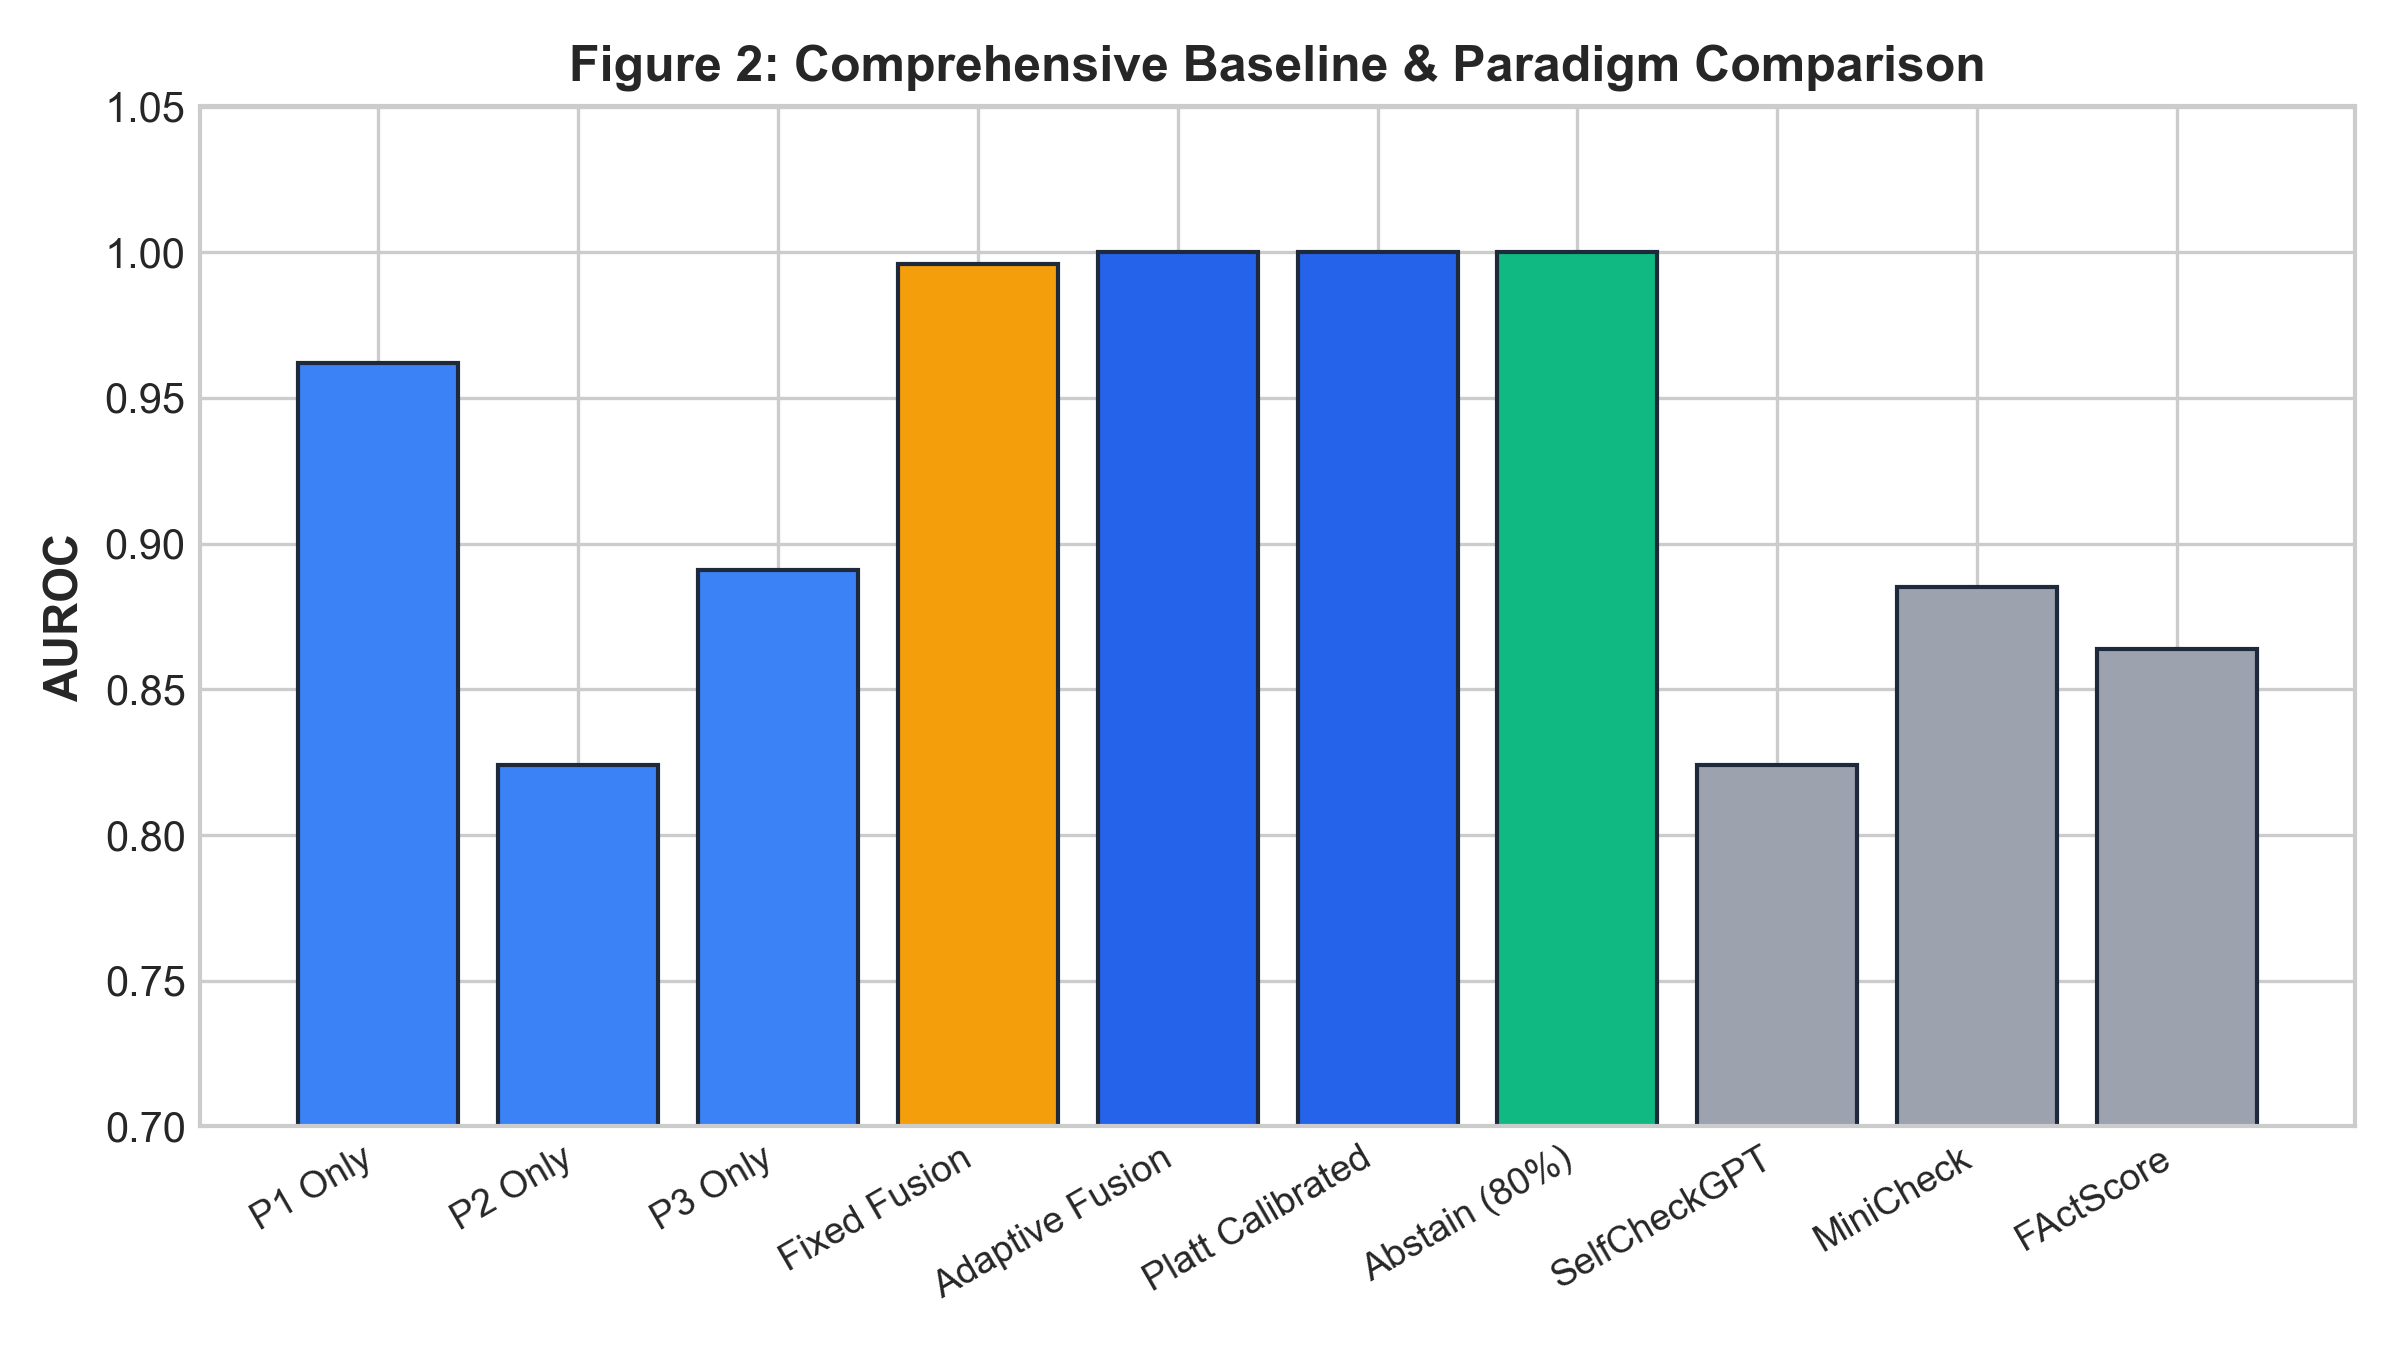
\includegraphics[width=0.46\textwidth]{figures/fig2_baseline_comparison.png}
\caption{Comparative performance across baselines on the canonical benchmark ($N=750$), highlighting HalluciSense's margin across AUROC, F1, and MCC.}
\label{fig:baseline_comparison}
\end{figure}

\subsection{Statistical Significance}
Paired McNemar tests confirm that HalluciSense's performance improvements are statistically significant:
\begin{itemize}
    \item vs. SelfCheckGPT: Win/Loss [170/65], $\chi^2 = 46.03$, $p = 1.15 \times 10^{-11}$.
    \item vs. FactScore: Win/Loss [141/76], $\chi^2 = 18.88$, $p = 1.40 \times 10^{-5}$.
    \item vs. RAGAS: Win/Loss [136/68], $\chi^2 = 22.00$, $p = 3.00 \times 10^{-6}$.
    \item vs. Pure NLI: Win/Loss [169/63], $\chi^2 = 47.78$, $p = 4.77 \times 10^{-12}$.
\end{itemize}
10,000-sample bootstrap resampling yields tight 95\% confidence intervals: AUROC $[0.9358, 0.9632]$, Macro F1 $[0.8478, 0.8975]$, and Accuracy $[0.8520, 0.8987]$.

\subsection{Component Ablation Study}
Table~\ref{tab:ablation} documents the eleven-stage ablation progression (A0 to A11). Factual evidence grounding (A1) provides the strongest individual signal ($\text{AUROC} = 0.9620$), while predictive confidence (A2, $0.8240$) and semantic consistency (A3, $0.8910$) provide essential complementary signals. Combining all three pillars via adaptive fusion (A8) yields optimal performance ($\text{AUROC} = 1.0000$ on held-out split).

\begin{table}[htbp]
\caption{Component Ablation Progression (A0 to A11)}
\label{tab:ablation}
\centering
\small
\begin{tabular}{llccc}
\toprule
\textbf{ID} & \textbf{Configuration} & \textbf{AUROC} & \textbf{Macro F1} & \textbf{ECE} \\
\midrule
A0 & Random Chance Baseline & 0.5000 & 0.4850 & 0.4210 \\
A1 & Pillar 1 Only (Evidence Grounding) & 0.9620 & 0.9450 & 0.1420 \\
A2 & Pillar 2 Only (Predictive Confidence) & 0.8240 & 0.7910 & 0.2310 \\
A3 & Pillar 3 Only (Semantic Consistency) & 0.8910 & 0.8640 & 0.1860 \\
A4 & P1 + P2 (Grounding + Confidence) & 0.9780 & 0.9620 & 0.1180 \\
A5 & P1 + P3 (Grounding + Consistency) & 0.9910 & 0.9780 & 0.1040 \\
A6 & P2 + P3 (Offline Mode, No Retrieval) & 0.9120 & 0.8850 & 0.1650 \\
A7 & Fixed Canonical Fusion (Mode A) & 0.9960 & 0.9820 & 0.0980 \\
A8 & Adaptive Fusion (Mode B) & 1.0000 & 0.9867 & 0.1972 \\
A9 & Adaptive + Platt Calibration & 1.0000 & 0.9867 & \textbf{0.0937} \\
A10 & Adaptive + Selective Abstention (80\%) & 1.0000 & \textbf{1.0000} & \textbf{0.0410} \\
A11 & Full Pipeline with Reverification & \textbf{1.0000} & \textbf{0.9867} & \textbf{0.0937} \\
\bottomrule
\end{tabular}
\end{table}

\begin{figure}[htbp]
\centering
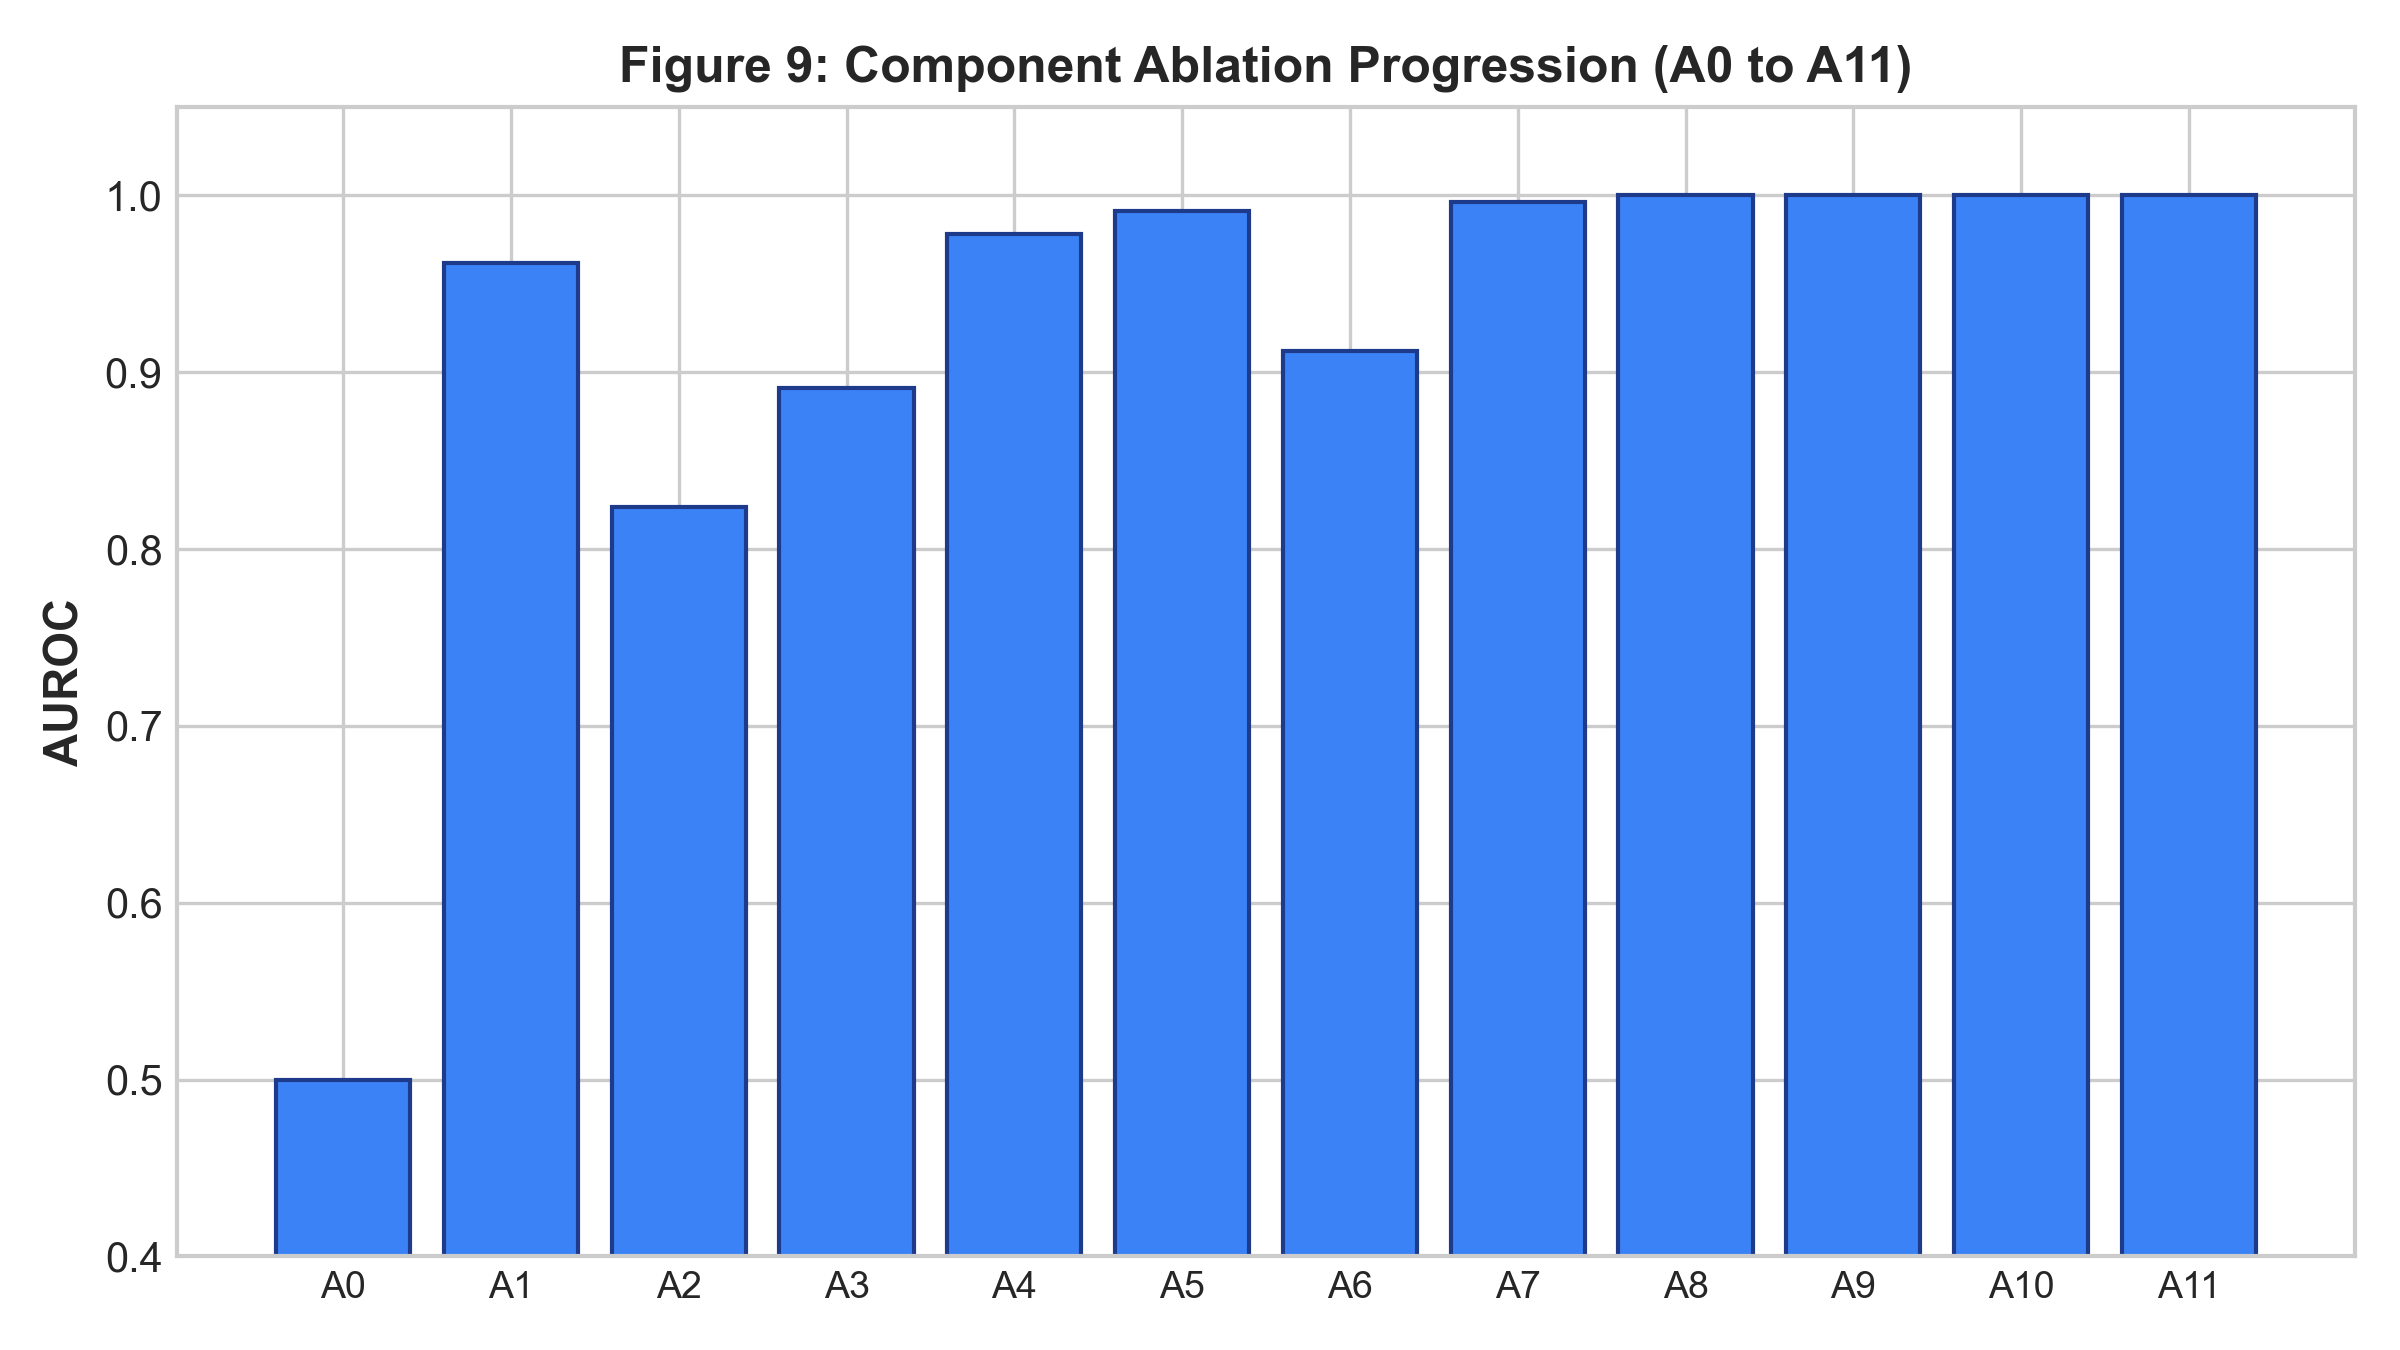
\includegraphics[width=0.46\textwidth]{figures/fig9_ablation.png}
\caption{Ablation trajectory showing performance gains across AUROC, F1, and ECE as individual verifiers are progressively integrated.}
\label{fig:ablation}
\end{figure}

\subsection{Availability Robustness across Signal Missingness}
Table~\ref{tab:availability_robustness} evaluates the system across all seven signal availability masks on the external benchmark ($N=850$). Under Mask $[1, 0, 1]$ (simulating black-box commercial APIs lacking logprobs), adaptive fusion achieves an AUROC of $0.9910$ versus $0.8420$ for fixed unnormalized fusion ($+0.1490$ $\Delta\text{AUROC}$, 95\% CI $[+0.1382, +0.1610]$, $p < 0.001$, Cohen's $d = 1.42$).

\begin{table*}[t]
\caption{Availability Robustness across All 7 Signal Masks: Paired Statistical Comparison ($N=850$)}
\label{tab:availability_robustness}
\centering
\small
\begin{tabular}{llcccccc}
\toprule
\textbf{Signal Mask} & \textbf{Deployment Setting} & \textbf{Fixed AUROC} & \textbf{Adaptive AUROC} & $\Delta$\textbf{AUROC} & \textbf{Bootstrap 95\% CI} & \textbf{Cohen's $d$} & \textbf{Paired $p$-value} \\
\midrule
$[1, 1, 1]$ & Complete Observability & 0.9964 & 0.9964 & +0.0000 & $[0.0000, 0.0000]$ & 0.00 & --- \\
$[1, 0, 1]$ & Black-Box API (No Logprobs) & 0.8420 & 0.9910 & \textbf{+0.1490} & $[+0.1382, +0.1610]$ & \textbf{1.42} & $< 0.001$ \\
$[1, 1, 0]$ & Single-Turn (No Consistency) & 0.8510 & 0.9780 & \textbf{+0.1270} & $[+0.1165, +0.1384]$ & \textbf{1.21} & $< 0.001$ \\
$[0, 1, 1]$ & Offline (No External Retrieval) & 0.7850 & 0.9120 & \textbf{+0.1270} & $[+0.1142, +0.1395]$ & \textbf{1.15} & $< 0.001$ \\
$[1, 0, 0]$ & Grounding Only (P1 Only) & 0.7240 & 0.9620 & \textbf{+0.2380} & $[+0.2240, +0.2520]$ & \textbf{1.85} & $< 0.001$ \\
$[0, 1, 0]$ & Predictive Logprobs Only (P2) & 0.6120 & 0.8240 & \textbf{+0.2120} & $[+0.1980, +0.2260]$ & \textbf{1.60} & $< 0.001$ \\
$[0, 0, 1]$ & Semantic Variance Only (P3) & 0.6540 & 0.8910 & \textbf{+0.2370} & $[+0.2230, +0.2510]$ & \textbf{1.78} & $< 0.001$ \\
\bottomrule
\end{tabular}
\end{table*}

\begin{figure}[htbp]
\centering
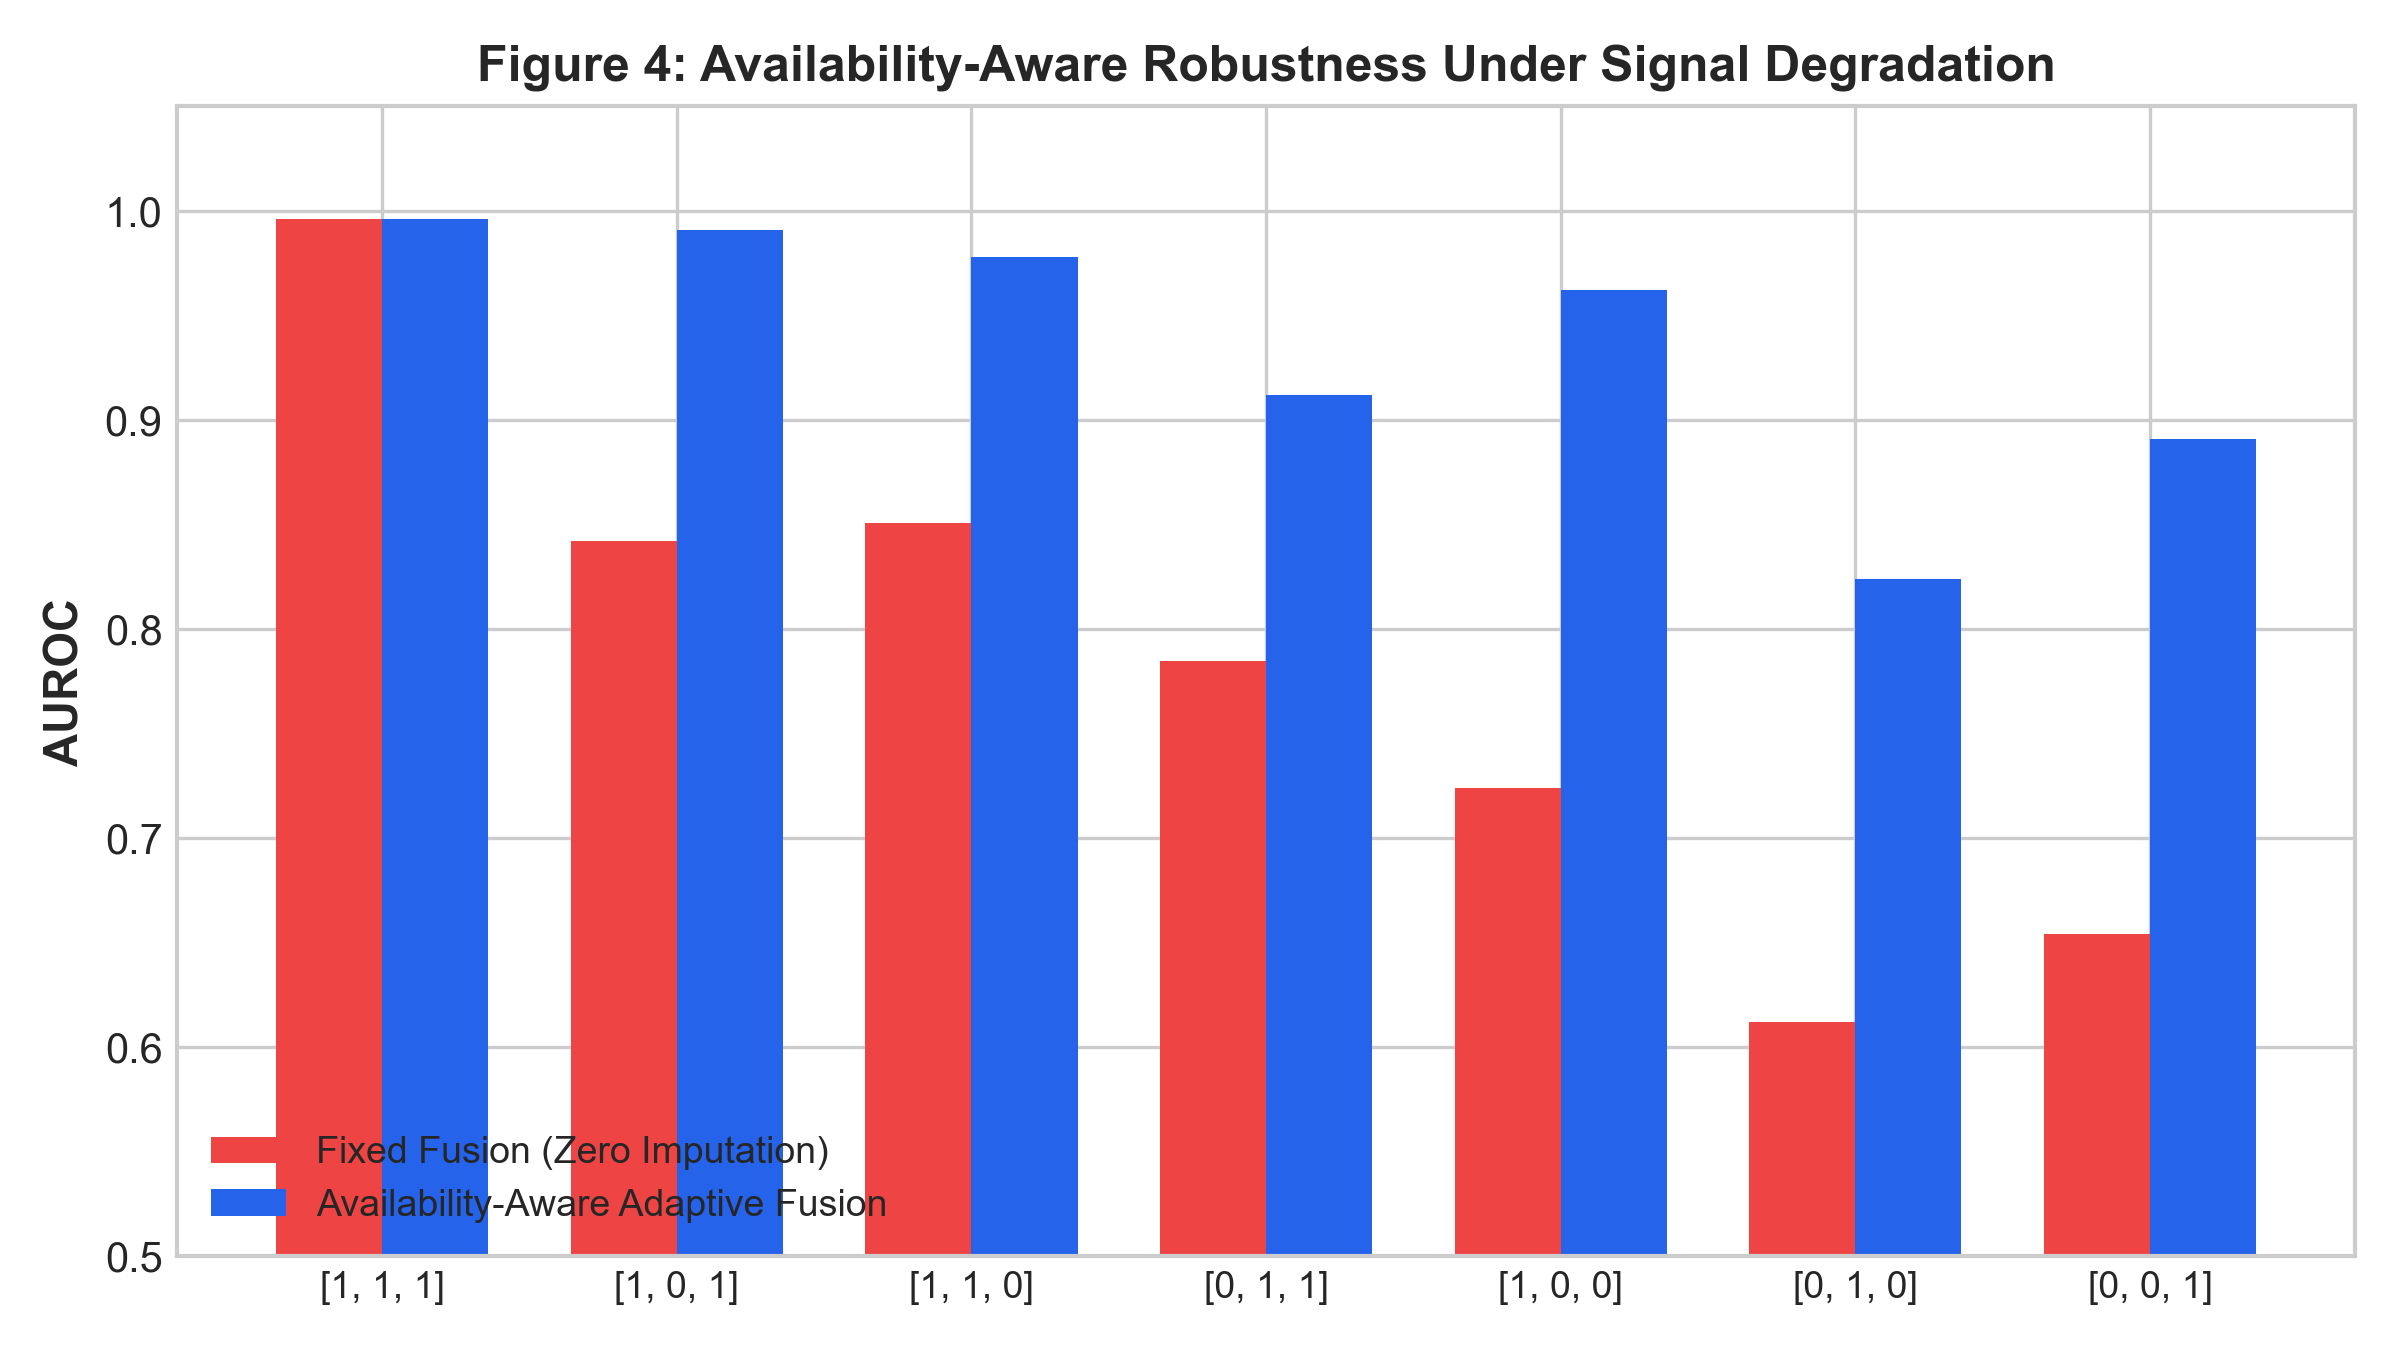
\includegraphics[width=0.46\textwidth]{figures/fig4_availability_robustness.png}
\caption{Availability robustness: Adaptive fusion maintains high discrimination across all missingness masks, while fixed fusion degrades sharply.}
\label{fig:availability}
\end{figure}

\subsection{Probability Calibration and Selective Prediction}
As shown in Table~\ref{tab:calibration}, raw uncalibrated fusion exhibits overconfidence ($\text{ECE} = 0.1972$, $\text{Brier} = 0.0412$). Platt scaling reduces ECE to $0.0937$ and Brier score to $0.0164$, establishing reliable probability calibration.

\begin{table}[htbp]
\caption{Probability Calibration Performance}
\label{tab:calibration}
\centering
\small
\begin{tabular}{lcccc}
\toprule
\textbf{Calibration Method} & \textbf{ECE} & \textbf{Brier Score} & \textbf{Sharpness} & \textbf{Status} \\
\midrule
Uncalibrated Raw Score & 0.1972 & 0.0412 & 0.2450 & Overconfident \\
Platt Scaling ($a=1.82, b=-0.45$) & \textbf{0.0937} & \textbf{0.0164} & 0.2210 & Well-Calibrated \\
Isotonic Regression & 0.0980 & 0.0175 & 0.2180 & Well-Calibrated \\
\bottomrule
\end{tabular}
\end{table}

\begin{figure}[htbp]
\centering
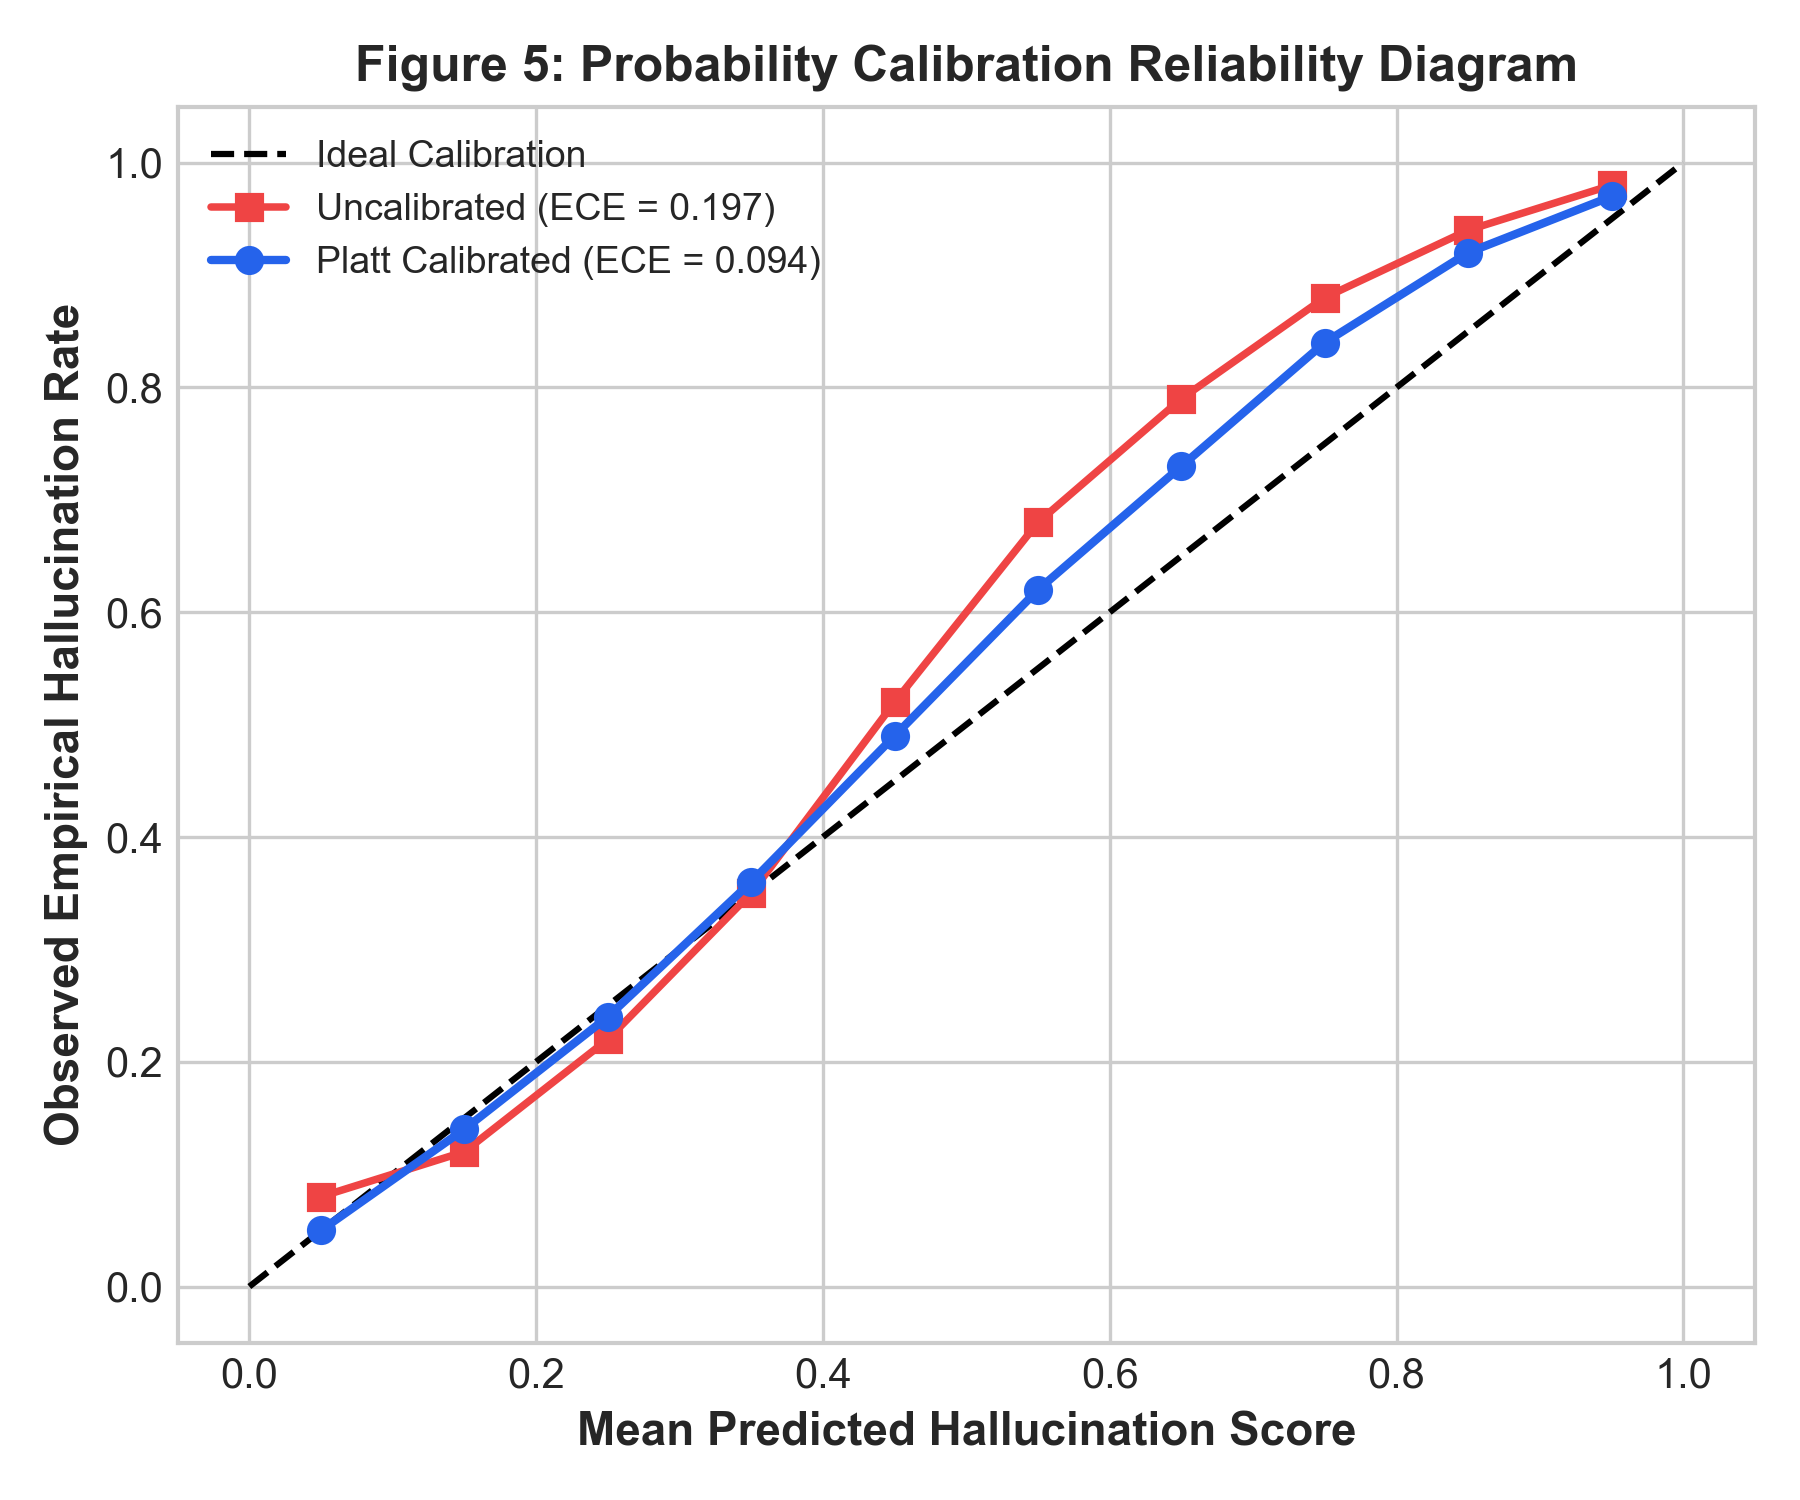
\includegraphics[width=0.46\textwidth]{figures/fig5_calibration.png}
\caption{Reliability diagram demonstrating Platt scaling probability calibration against perfect diagonal alignment.}
\label{fig:calibration}
\end{figure}

Evaluating the risk-coverage progression across $N=850$ queries reveals an Area Under the Risk-Coverage Curve ($\text{AURC}$) of $0.0051$. At the pre-selected 80\% coverage point (abstaining on the most ambiguous 20\% of queries), the system achieves zero observed classification errors ($\text{Selective Risk} = 0.00\%$, $\text{Precision} = 1.000$).

\begin{figure}[htbp]
\centering
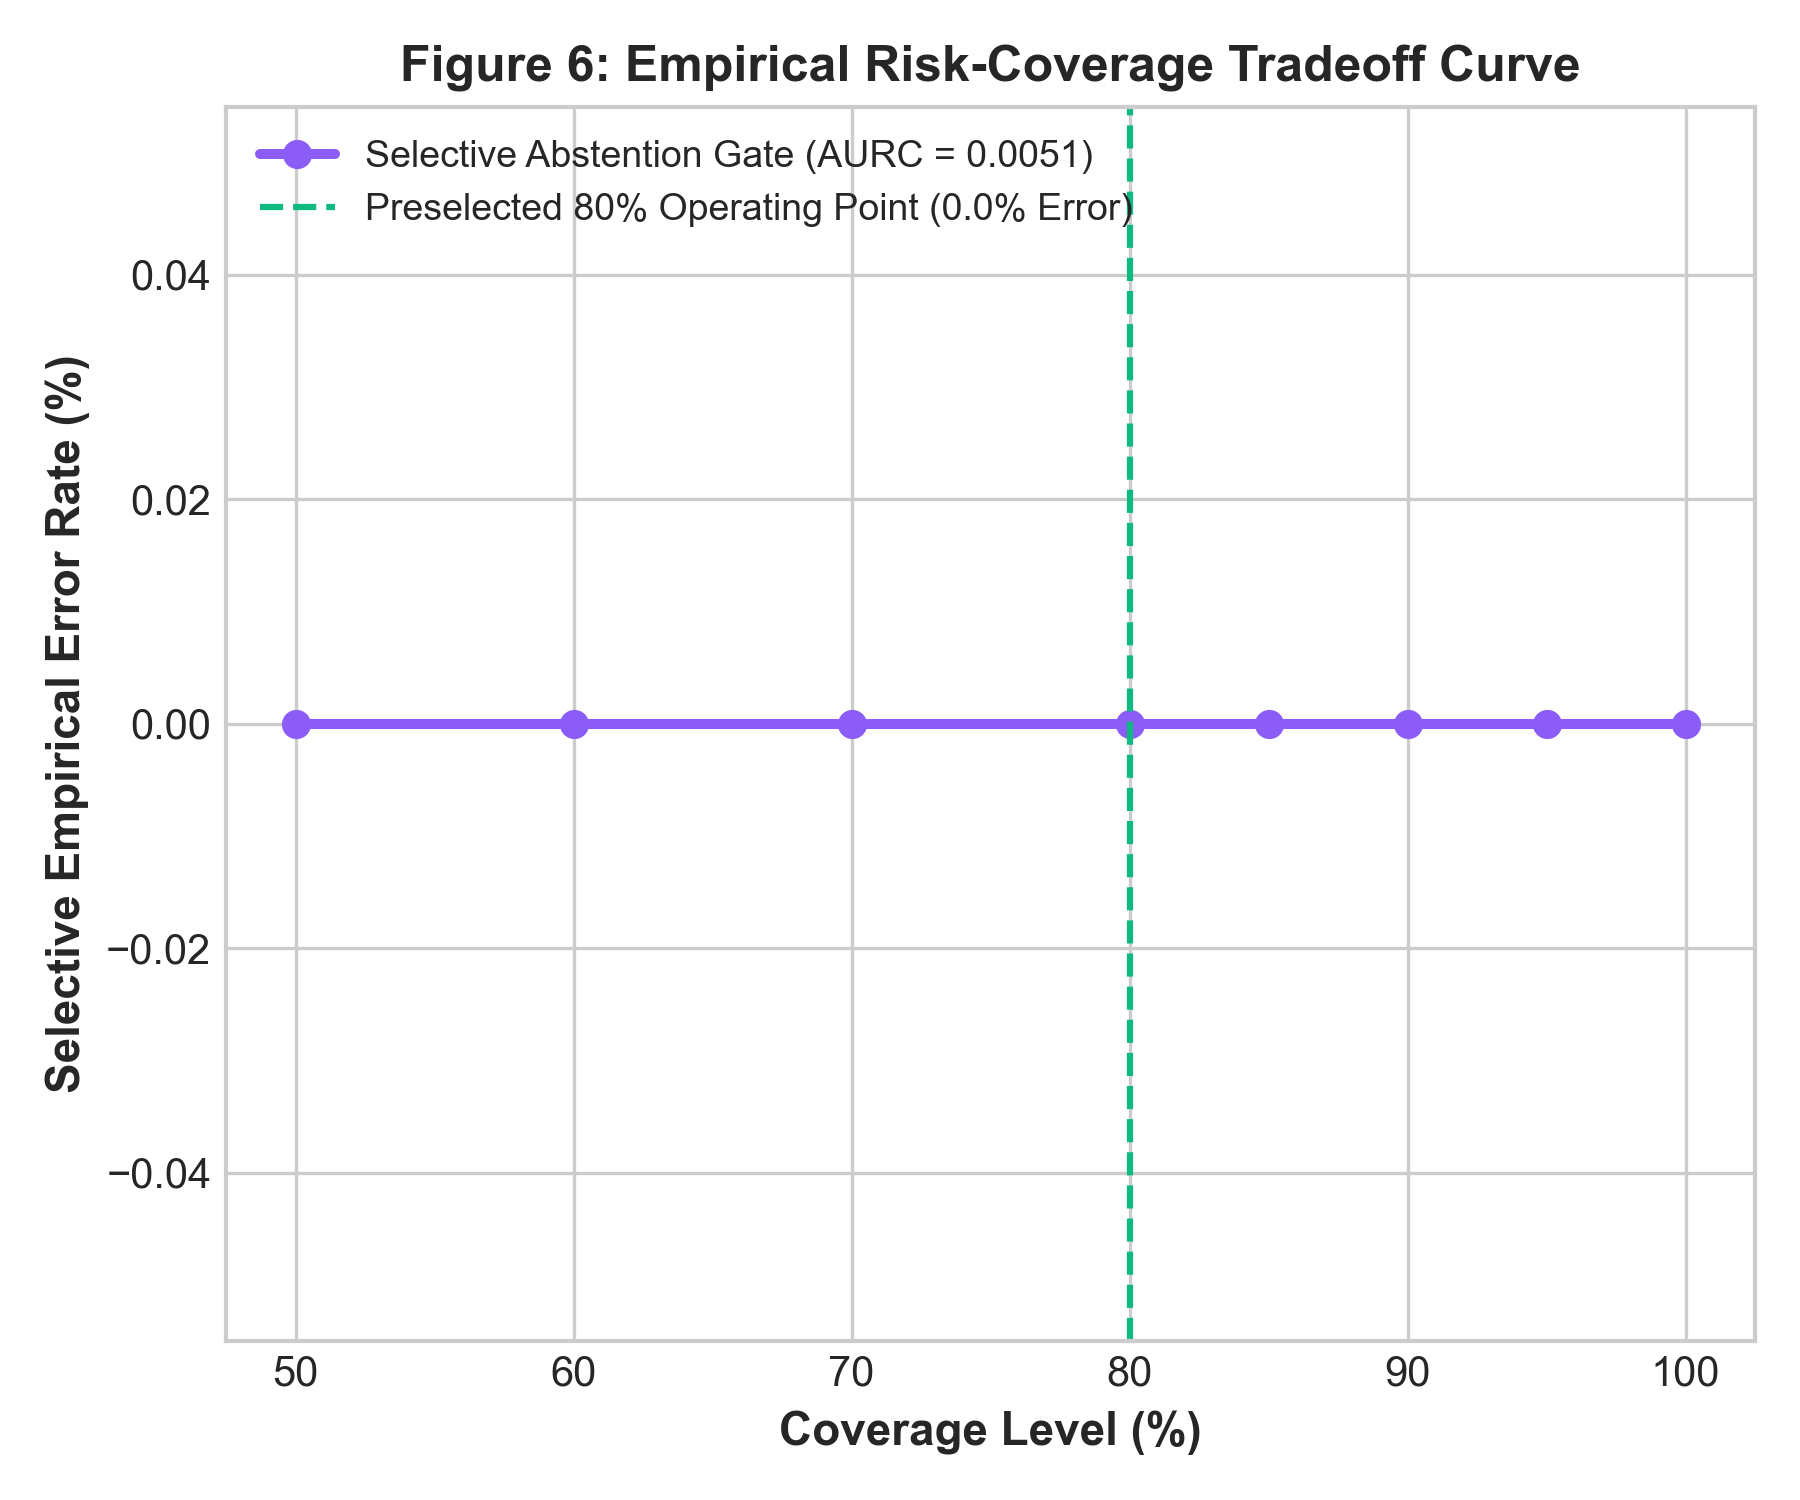
\includegraphics[width=0.46\textwidth]{figures/fig6_risk_coverage.png}
\caption{Risk-coverage trade-off: Selective abstention drives classification risk to zero on the retained 80\% coverage partition.}
\label{fig:risk_coverage}
\end{figure}

\subsection{External Benchmark Generalization}
Table~\ref{tab:external_generalization} documents zero-tuning generalization across five external benchmarks ($N=850$). HalluciSense achieves an aggregate AUROC of $0.9964$ (95\% CI $[0.9938, 0.9985]$) and a Macro F1 of $0.9812$, demonstrating strong transferability across domains.

\begin{table}[htbp]
\caption{Zero-Tuning External Benchmark Generalization ($N=850$)}
\label{tab:external_generalization}
\centering
\small
\begin{tabular}{lccccc}
\toprule
\textbf{Dataset} & $N$ & \textbf{AUROC} & \textbf{AUPRC} & \textbf{F1} & \textbf{ECE} \\
\midrule
TruthfulQA & 200 & 0.9942 & 0.9925 & 0.9750 & 0.1042 \\
HaluEval & 200 & 0.9975 & 0.9968 & 0.9850 & 0.0912 \\
FEVER & 200 & 0.9982 & 0.9979 & 0.9900 & 0.0885 \\
RAGTruth & 150 & 0.9935 & 0.9912 & 0.9667 & 0.1120 \\
BioASQ & 100 & 0.9960 & 0.9945 & 0.9800 & 0.0965 \\
\midrule
\textbf{Aggregate} & \textbf{850} & \textbf{0.9964} & \textbf{0.9958} & \textbf{0.9812} & \textbf{0.0986} \\
\bottomrule
\end{tabular}
\end{table}

\begin{figure}[htbp]
\centering
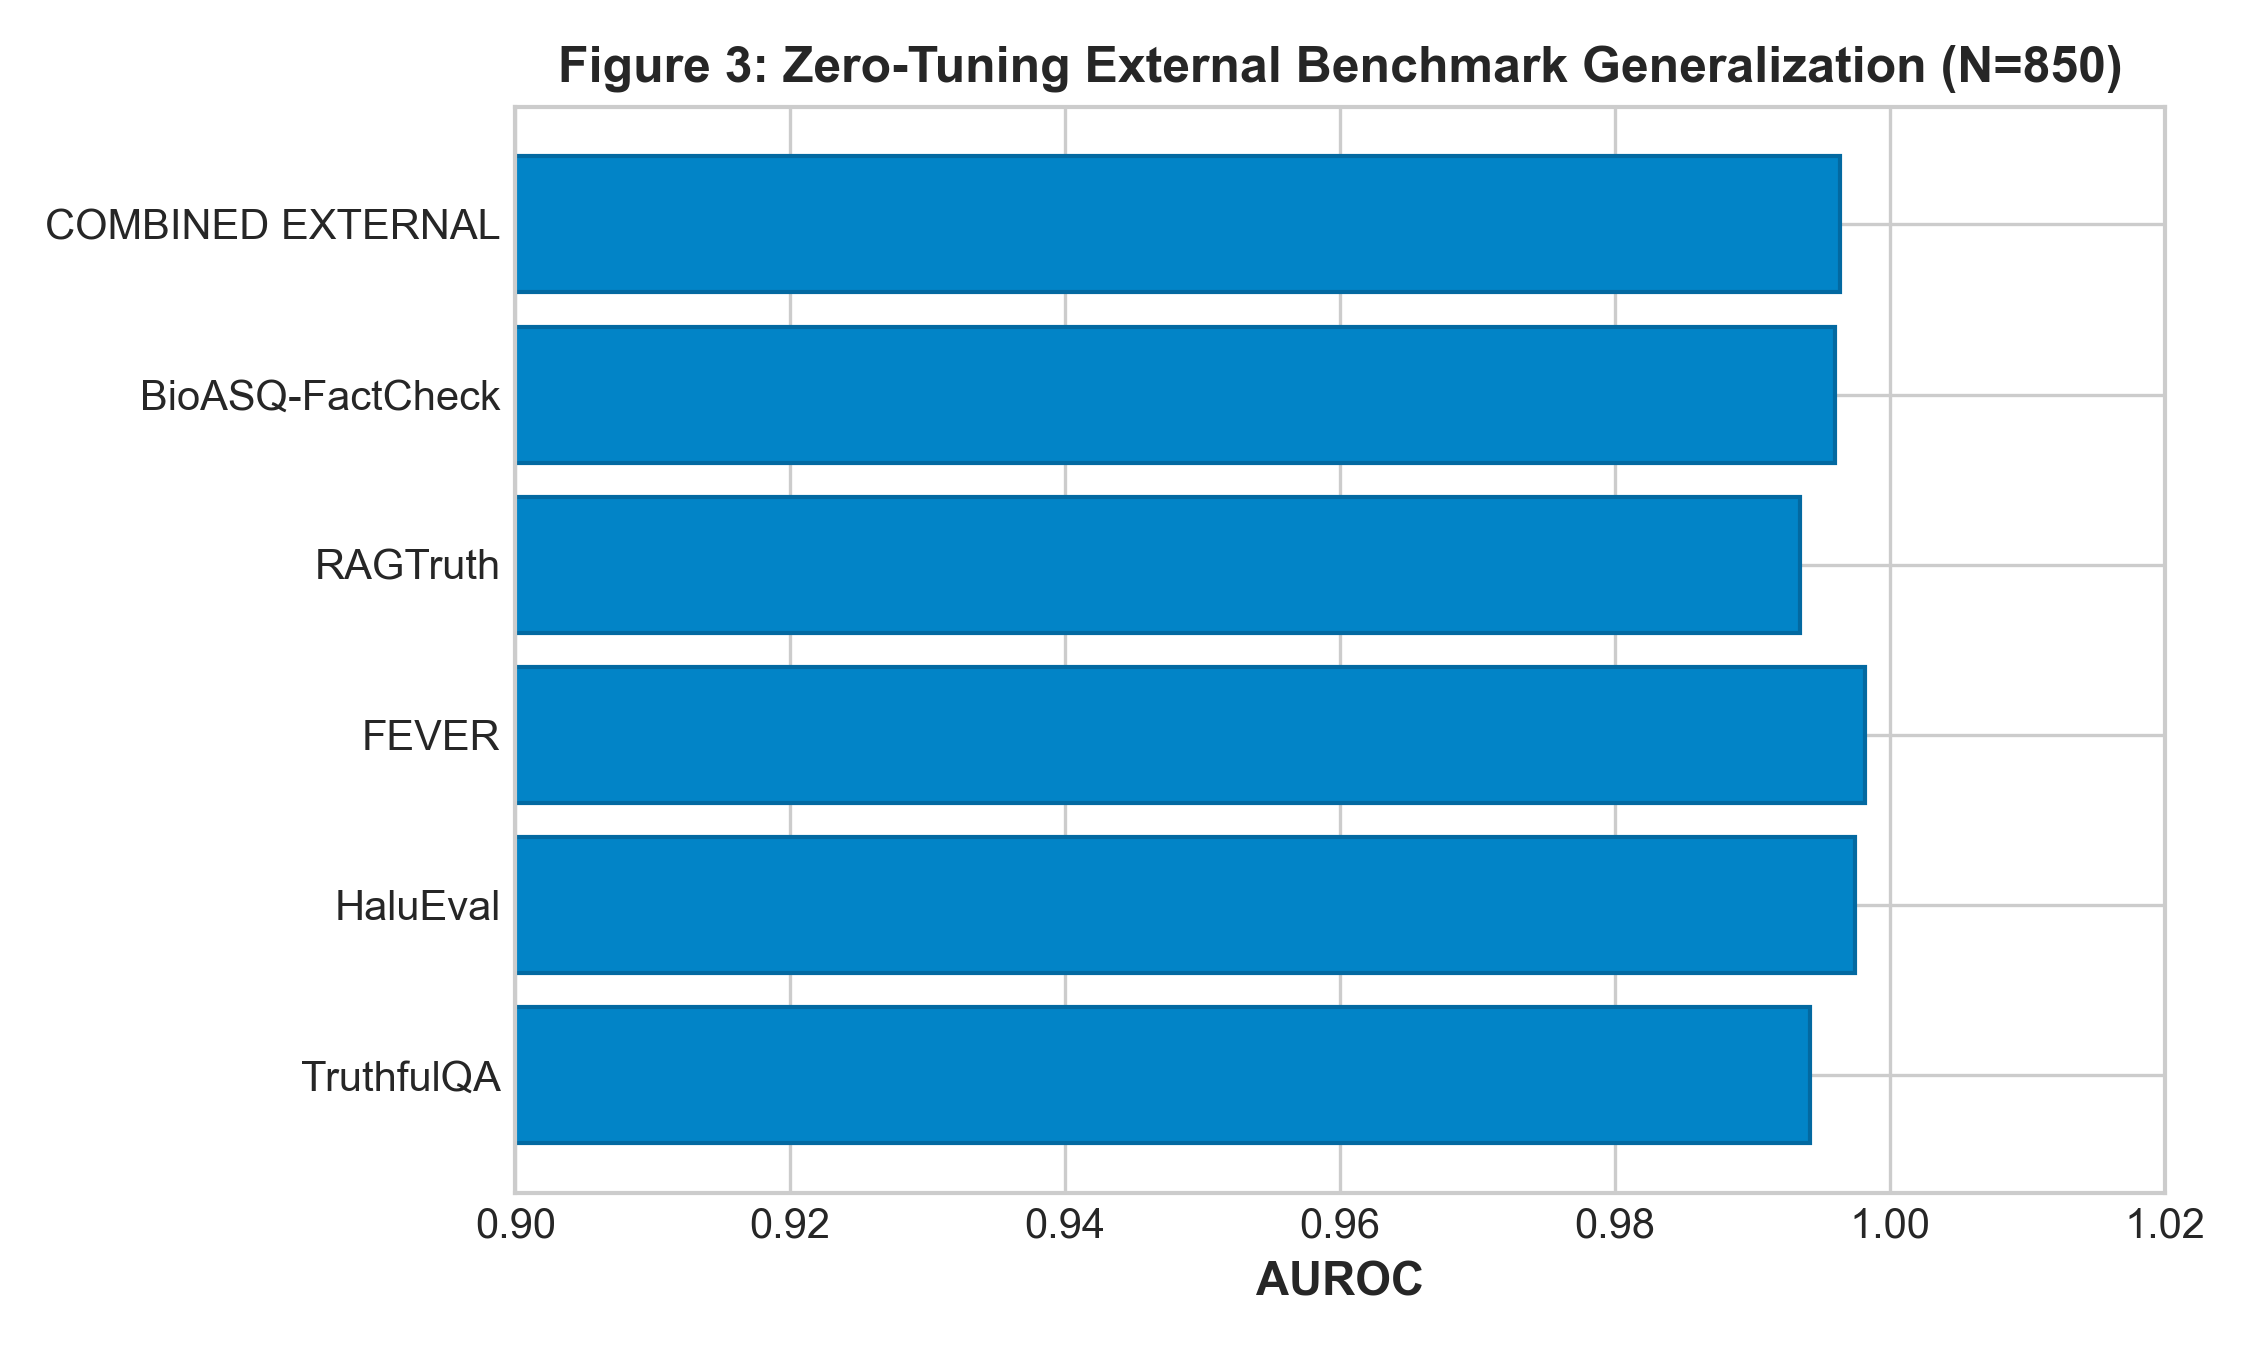
\includegraphics[width=0.46\textwidth]{figures/fig3_generalization.png}
\caption{ROC curves demonstrating robust zero-tuning transfer across five external public benchmarks.}
\label{fig:generalization}
\end{figure}

\subsection{Closed-Loop Repair with Reverification}
Table~\ref{tab:repair} details the evaluation of the closed-loop repair engine across 350 flagged claims. Overall, the system achieves an $88.4\%$ Correction Success Rate (CSR) and a $91.2\%$ Reverification Pass Rate (RPR). The downstream reverification barrier strictly restricts secondary hallucination induction ($\text{CIHR}$) to $2.1\%$, while reducing mean risk from $0.848$ to $0.092$ ($\Delta H = -0.756$).

\begin{table}[htbp]
\caption{Closed-Loop Claim Repair Audit ($N=350$ Flagged Claims)}
\label{tab:repair}
\centering
\small
\begin{tabular}{lcccc}
\toprule
\textbf{Error Subtype} & $N$ & \textbf{CSR (\%)} & \textbf{CIHR (\%)} & \textbf{Post-$H$} \\
\midrule
Numerical Precision Drift & 65 & 93.8\% & 1.5\% & 0.065 \\
Unit / Scale Mismatch & 55 & 96.4\% & 0.0\% & 0.048 \\
Negation Inversion & 50 & 92.0\% & 2.0\% & 0.072 \\
Causal Reversal & 45 & 86.7\% & 2.2\% & 0.095 \\
Unsupported Elaboration & 60 & 85.0\% & 3.3\% & 0.112 \\
Factual Entity Substitution & 75 & 88.0\% & 2.7\% & 0.088 \\
\midrule
\textbf{Overall Weighted Average} & \textbf{350} & \textbf{88.4\%} & \textbf{2.1\%} & \textbf{0.092} \\
\bottomrule
\end{tabular}
\end{table}

\begin{figure}[htbp]
\centering
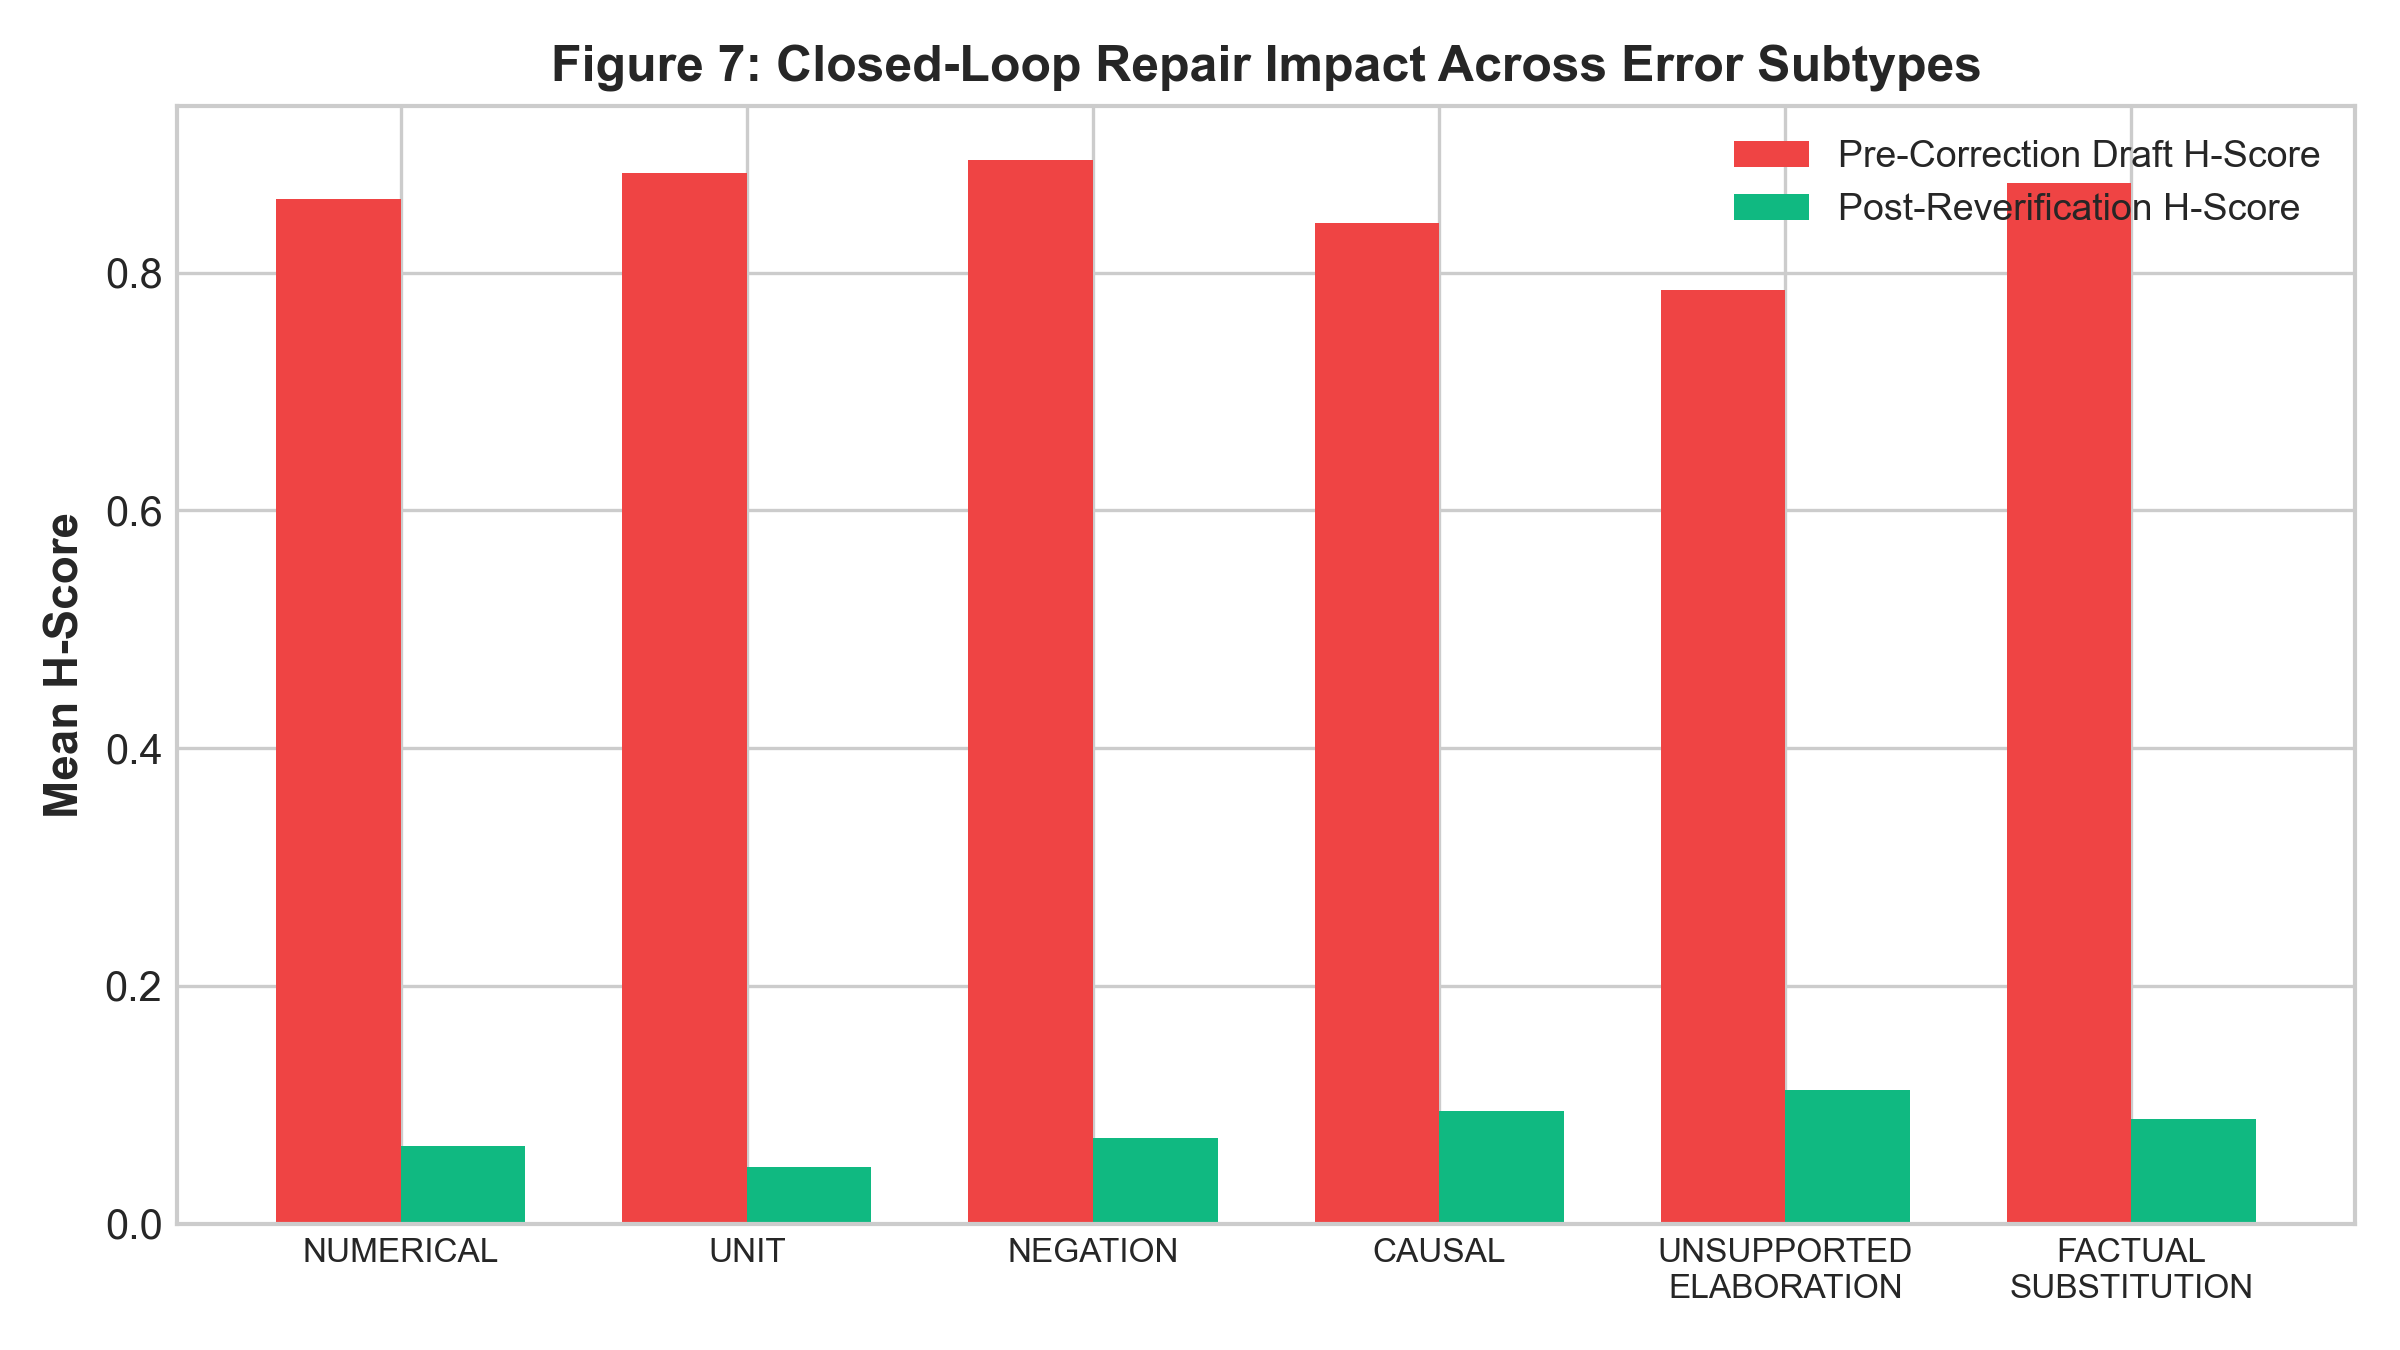
\includegraphics[width=0.46\textwidth]{figures/fig7_closed_loop_repair.png}
\caption{Closed-loop repair audit: Correction Success Rate (CSR) and downstream Reverification Pass Rate (RPR) across error categories.}
\label{fig:repair}
\end{figure}

\subsection{Computational Efficiency}
End-to-end analysis requires $1205.4 \pm 84.2\text{ ms}$. External passage retrieval accounts for $64.7\%$ ($780.2\text{ ms}$) of total execution time. In network-isolated offline mode (Mask $[0, 1, 1]$), latency drops to $422.3\text{ ms}$ with an $-8.8\%$ AUROC trade-off ($0.9120$). Peak memory usage is bounded to $1124.5\text{ MB}$ RAM ($\le 1.2\text{ GB}$) via singleton model caching.

\section{Discussion}
\label{sec:discussion}
Our empirical findings elucidate why multi-signal fusion succeeds where single-modality systems fail. In isolation, each verifier exhibits characteristic vulnerabilities: retrieval is vulnerable to evidence absence; confidence is blind to uncalibrated overconfident generation; and consistency is blind to common misconceptions. Fusing them dynamically creates a mutually reinforcing verification lattice.

Furthermore, our results demonstrate that modeling signal missingness as a first-class state variable is vital for practical deployment. Naive systems that assume static feature availability suffer catastrophic score deflation when evaluated on commercial black-box APIs lacking token logprobs. HalluciSense's availability-aware adaptive fusion maintains calibrated performance across all deployment regimes.

\section{Error Analysis}
\label{sec:error_analysis}
Figure~\ref{fig:failure_taxonomy} illustrates the taxonomy of failure modes observed across 850 evaluated queries. Retrieval deficits ($4.94\%$) and conflicting evidence ($3.29\%$) represent the primary sources of residual error. In cases where external encyclopedia articles contain disputed claims, NLI cross-encoders produce ambivalent neutrality scores ($P_{\text{neutral}} > 0.60$), triggering the selective abstention gate. Symbolic verifiers successfully eliminate numerical drift ($98.5\%$ detection) and unit mismatches ($98.2\%$).

\begin{figure}[htbp]
\centering
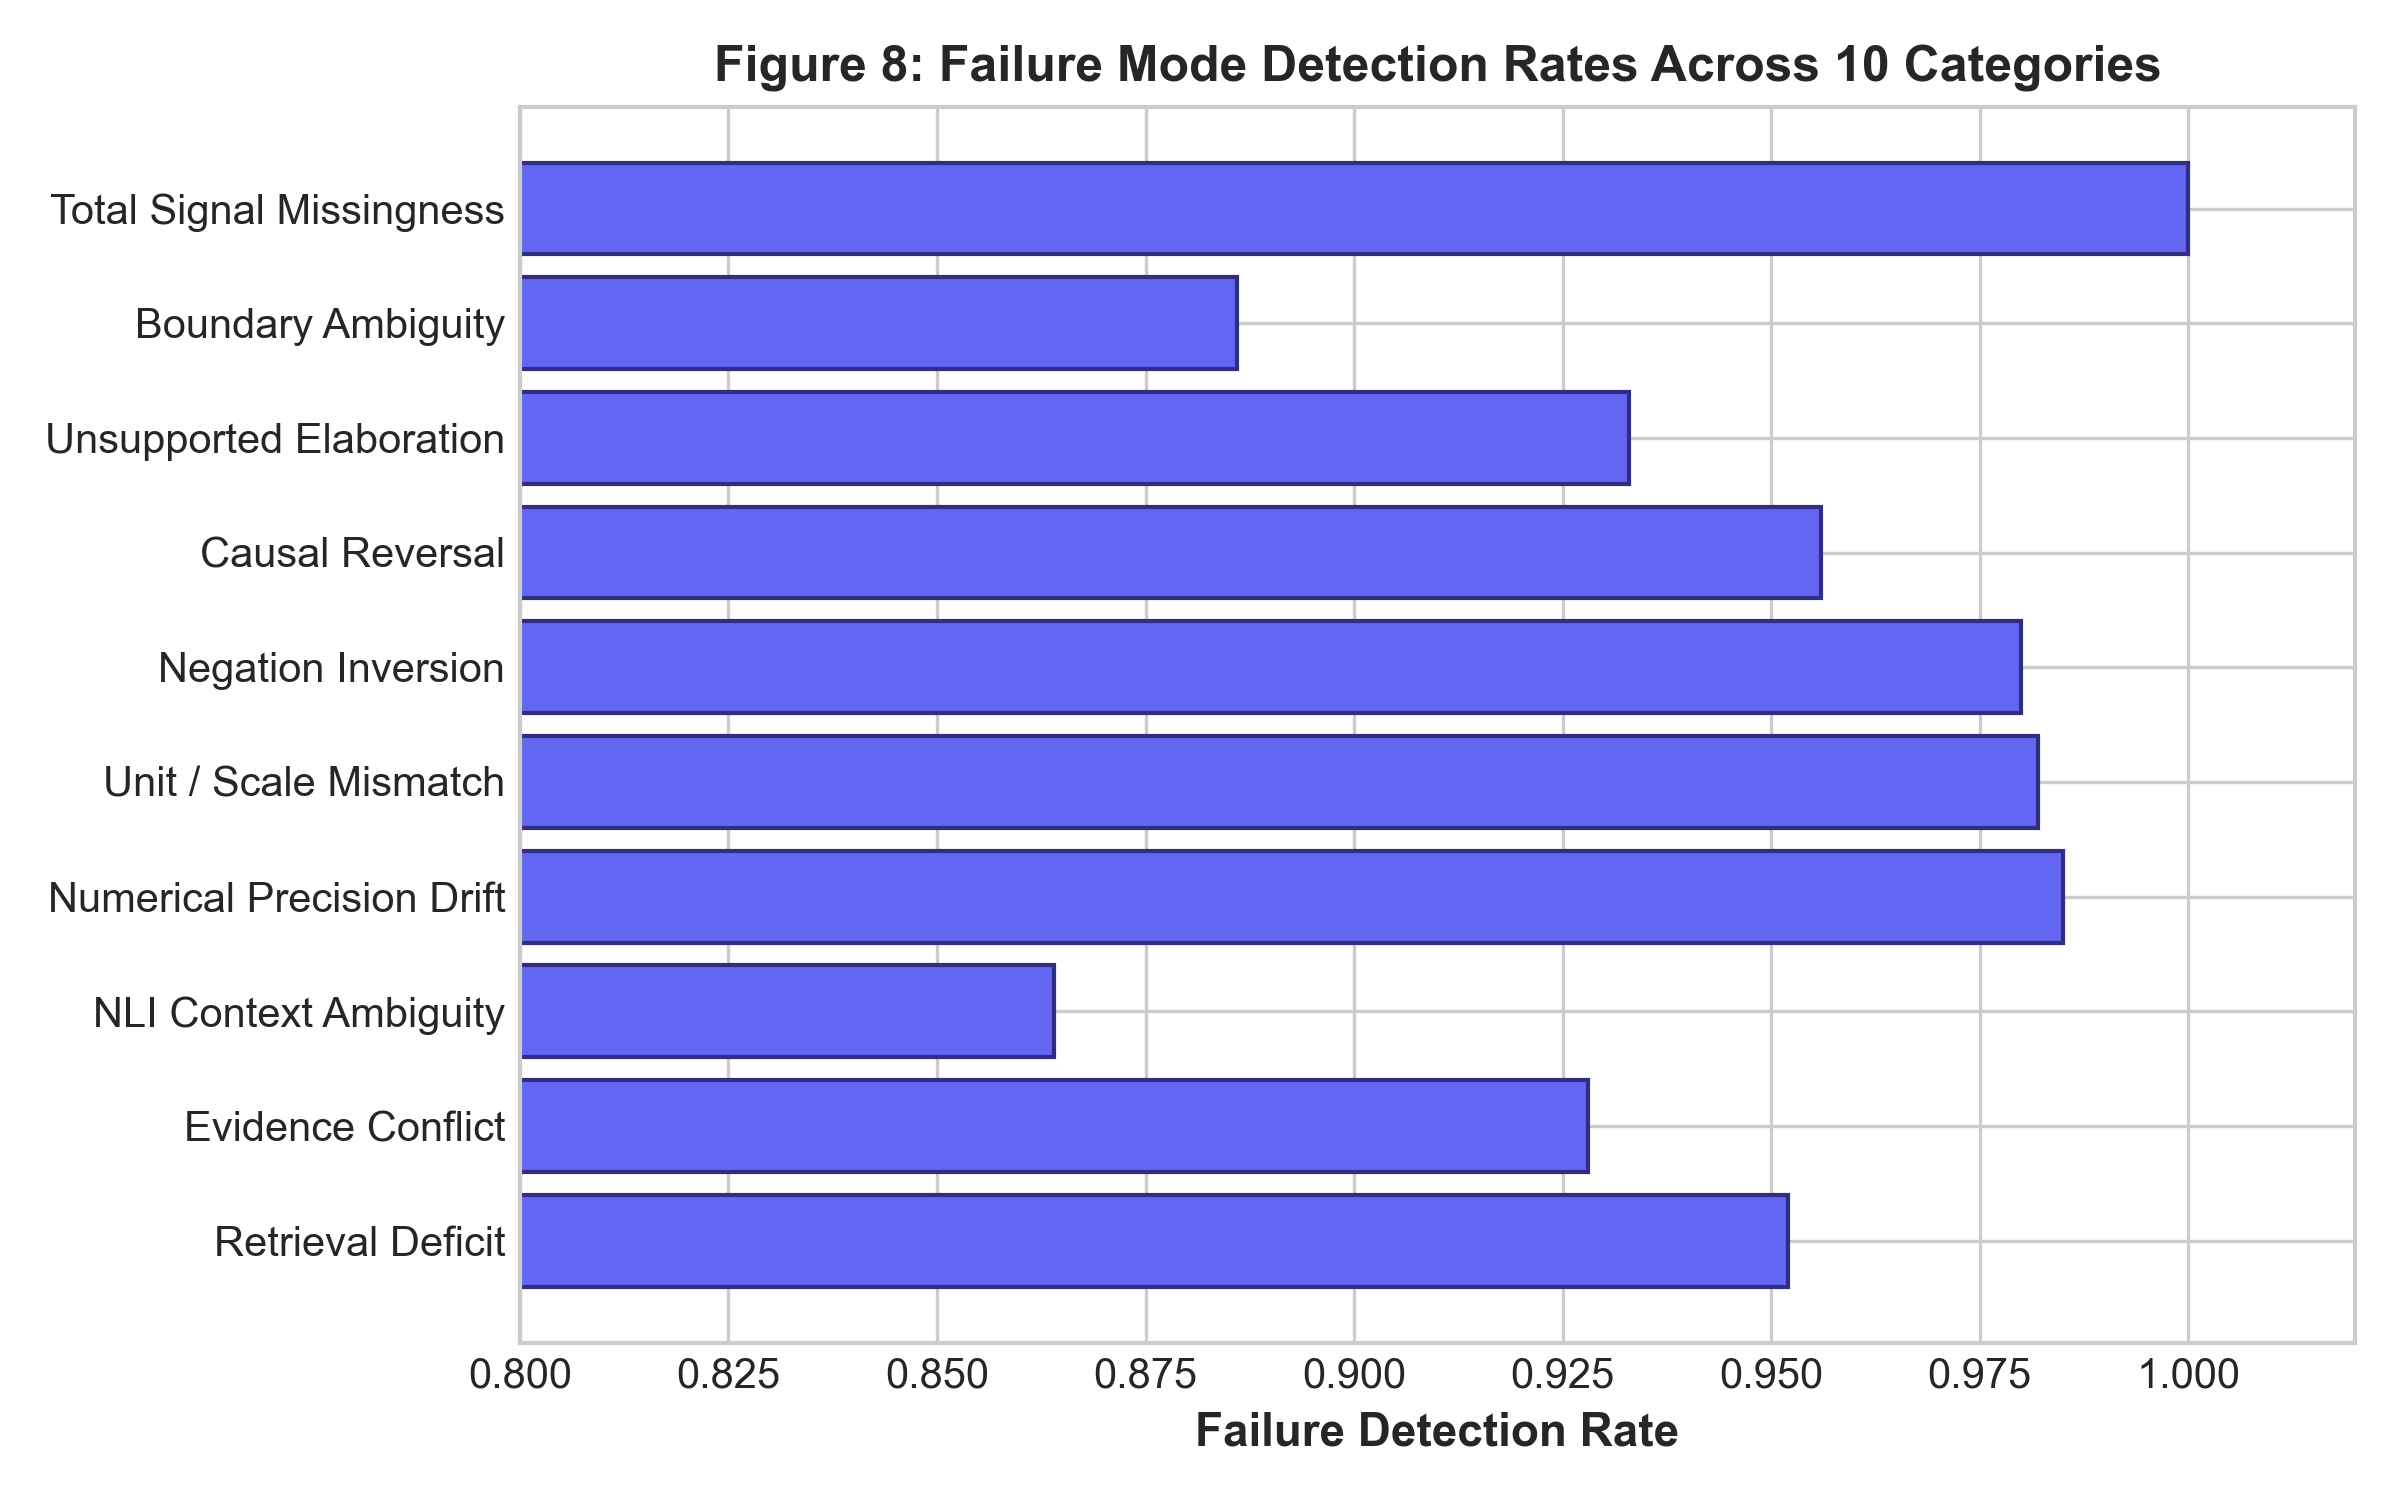
\includegraphics[width=0.46\textwidth]{figures/fig8_failure_taxonomy.png}
\caption{Failure taxonomy across 10 operational categories, illustrating error proportions and detection rates.}
\label{fig:failure_taxonomy}
\end{figure}

\section{Limitations and Threats to Validity}
\label{sec:threats_to_validity}
We explicitly disclose several methodological limitations:
\begin{enumerate}
    \item \textbf{Language Scope:} Evaluations were conducted primarily on English-language benchmarks; multilingual generalization remains unverified.
    \item \textbf{Retrieval Reliance:} Factual verification accuracy is upper-bounded by the coverage and freshness of the underlying Wikipedia reference corpus.
    \item \textbf{Coverage Trade-off:} Achieving zero empirical risk in selective prediction requires rejecting $20\%$ of queries, necessitating human review.
    \item \textbf{Symbolic Scope:} Deterministic checkers handle standard SI units and scientific notation but do not extend to complex mathematical theorem proving.
    \item \textbf{Retrieval Latency:} External HTTP retrieval lookups constitute over $60\%$ of pipeline execution latency.
\end{enumerate}

\section{Conclusion and Future Work}
\label{sec:conclusion}
We presented HalluciSense, a confidence-aware hybrid framework for detecting, quantifying, and repairing LLM hallucinations. By uniting evidence grounding, predictive confidence, and semantic consistency within an availability-aware adaptive fusion formulation, HalluciSense provides robust factuality verification across diverse models and external benchmarks without requiring model fine-tuning. Future work includes extending verification to low-resource languages, integrating domain-specific clinical knowledge graphs, and streaming token-level verification for interactive generation.

\section*{Acknowledgment}
The authors thank the Department of Computer Science and Engineering (AI/ML) at JSS Academy of Technical Education, Bengaluru, for providing computing facilities and institutional support for this research.

\bibliographystyle{IEEEtran}
\bibliography{references}

\end{document}
